\documentclass{rapportENSCP}
\usepackage{lipsum}
\usepackage{tabularx} 
\usepackage{xspace}
\usepackage{multirow}
\usepackage{makecell}
\usepackage{graphicx}

\title{Rapport Stage Ouvrier- Template} %Thanks for Rapport CentraleSupelec - Template, By Axel Poupart-Lafarge
\begin{document}
\newcommand{\YGG}{$Y_3Ga_5O_{12}\xspace $ }
\newcommand{\YIG}{$Y_3Fe_5O_{12}\xspace $ }
\newcommand{\YAG}{$Y_3Al_5O_{12}\xspace $ }



%----------- Informations du rapport ---------

\logoentreprise{logos/logoIRCP.png}

\titre{Rapport de stage en laboratoire} % Titre du fichier

\mention{Stage expérimental en laboratoire} % Nom de la Mention
%\trigrammemention{Master IA} % Pour le bas de la page
\master{Cycle Ingénieur} % Nom du master
%\filiere{Filière Management de projet et Transformation} % Nom de la filière

\eleve{Alban Laborde-Laulhé}

\dates{24 septembre 2024 - 19 décembre 2024}

% Informations tuteurs écoles
\tuteurecole{
    \textsc{Pierre Haquette} \\
    pierre.haquette@chimieparistech.psl.eu
} 

\tuteurentreprise{
    \textsc{Pascal Loiseau} \\
    pascal.loiseau@chimieparistech.psl.eu \\
    \textsc{Alban Ferrier} \\
    alban.ferrier@chimieparistech.psl.eu
}

%----------- Initialisation -------------------
        
\fairemarges %Afficher les marges
\fairepagedegarde %Créer la page de garde

%----------- Abstract -------------------
%\vspace*{\stretch{1}}
%\begin{center}
%	\begin{abstract}
%        \lipsum[1]
%        \rule{\linewidth}{0.2 mm} \\[0.4 cm]
%        \begin{center}\textbf{Summary :}\end{center} 
%        \lipsum[2]
%    \end{abstract}
%\end{center}
%\vspace*{\stretch{1}}
%\newpage

%------------ Table des matières ----------------
\setcounter{figure}{0}

\tabledematieres % Créer la table de matières

%------------ Corps du rapport ----------------


%------------ Introduction ----------------

\section{Remerciements} 
Je tiens tout d’abord à remercier chaleureusement mes deux encadrants, Pascal Loiseau et Alban Ferrier, pour leur accompagnement tout au long de ce stage. Leur patience, leur pédagogie et leur disponibilité, malgré des emplois du temps très chargés, ont été précieuses pour répondre à mes nombreuses questions et m’assister lors de mes premières manipulations expérimentales.

Je souhaite ensuite exprimer ma reconnaissance à toute l’équipe MPOE pour son accueil bienveillant, et tout particulièrement à Slimane Raissi pour sa gentillesse, ses explications toujours claires et son soutien précieux dans la surveillance de certaines expériences lorsque je n’étais pas disponible, ainsi qu’à Nicolas Caraud pour sa patience et ses conseils avisés concernant le fonctionnement des différents appareils du laboratoire. Merci également à Alix Guerber pour son énergie et sa bonne humeur, et à Jean-François Engrand qui, non content d’avoir la réponse à peu près n’importe quel problème, sait aussi taper très fort – ce qui est pratique quand on veut casser des trucs.

Merci également à l’ensemble du personnel de l’IRCP, qui m’a chaleureusement accueilli et apporté son aide précieuse tout au long de ces trois mois. Enfin, mes remerciements vont aussi à Pierre Haquette et Philippe Vernazobres, représentants de l’école, qui m’ont permis de réaliser ce stage au sein de cette formidable équipe.

\newpage

\section{Abréviations}
\begin{itemize}
    \item \textbf{YAG : } Yttrium Aluminium Garnet (\YAG)
    \item \textbf{YGG : } Yttrium Gallium Garnet (\YIG)
    \item \textbf{YIG : } Yttrium Iron Garnet (\YGG)
    \item \textbf{YIGG : }Mélange contenant en proportions molaires 50\% de YGG et 50\% de YIG
    \item \textbf{DRX : }Diffraction des Rayons X
    
\end{itemize}
\section{Résumé}
Ce rapport présente les résultats d’un stage expérimental effectué au laboratoire MPOE de l'IRCP de Chimie ParisTech, portant sur la croissance en flux de grenats d’yttrium, notamment le YIG ($Y_3Fe_5O_{12}$) et le YGG ($Y_3Ga_5O_{12}$). L’objectif principal était d’évaluer la faisabilité et les conditions optimales de croissance de ces grenats dans deux systèmes de flux : $BaO-B_2O_3-BaF_2$ et $BaO-B_2O_3-Na_2O$.

Deux démarches expérimentales complémentaires ont été suivies. La première consistait à tenter la croissance dirigée d’un monocristal de YGG par tirage à partir d’un germe cristallin. Cette approche n’a toutefois pas permis de détecter la formation du grenat recherché, malgré la présence d'une phase cristalline non identifiée.

La seconde approche, impliquant des essais systématiques de cristallisation dans différents flux avec diverses concentrations en grenats, s’est révélée plus concluante. Le grenat YIG a été systématiquement formé et détecté à des concentrations de 7,5\%, démontrant la robustesse du protocole établi. En revanche, la cristallisation du YGG s’est avérée plus délicate n’étant détectée  dans le flux à base de sodium ($BaO-B_2O_3-BaF_2$) uniquement lorsque la proportion molaire de grenat a été portée à 10%.

Ces travaux confirment donc la possibilité de croissance du grenat YGG en flux sous conditions strictement contrôlées, ouvrant la voie à des études ultérieures d’optimisation fine des paramètres expérimentaux pour l’obtention de monocristaux adaptés aux applications en optique et en magnétisme.

\section{Introduction et contexte de recherche}
Ce stage s'inscrit dans la continuité des travaux de Samuel Collange, portant sur l'étude de la croissance en flux des grenats, et plus particulièrement du YGG et du YIG, respectivement de formule : \YGG et \YIG.

Les grenats naturels, de formule $X_3Y_2(SiO_4)_3$ constituent un groupe de minéraux cristallins où X et Y sont deux cations de degré d'oxydation II et III. Par analogie, on classe en général les composés de formules $X_3Y_2(ZO_4)_3$ dans le groupe des grenats synthétiques. Plus concrètement, la plupart du temps les cations $Y$ et $Z$ sont les mêmes ce qui permet d'écrire ces grenats sous la formule simplifiée $X_3Y_5O_{12}$.
Plus particulièrement, certains grenats contenant de l'Yttrium ont révélé posséder des propriétés physiques particulièrement intéressantes notamment pour des utilisations lasers ou de la conservation d'information quantique. L'un des grenats les plus étudiés est le YAG (\YAG), il est notamment un amplificateur laser efficace quand il est dopé au néodyme (Nd:YAG). Cela est rendu possible par l'inactivité optique de l'Yttrium et de sa substitution possible avec des ions de terres rares grâce à son rayon ionique et sa charge électrique voisine. Il existe aujourd'hui des dérivés du YAG comme le YIG (\YIG) et le YGG (\YGG) où l'ion d'aluminium est respectivement remplacé par du Fer ou du Gallium. Le YIG est un isolant ferrimagnétique reconnu pour sa faible dissipation magnétique et sa capacité à produire un effet Faraday significatif. Tandis que le YGG pouvant également être dopé par des ions de terres rares tout en étant un matériau transparent est employé pour ses propriétés optiques ou pour l'information quantique.

\begin{figure}[h] % h = here (ici)
    \centering
    \includegraphics[width=0.7\textwidth]{figures/YIG_representation.png}
    \caption{Représentation d’une maille de YIG comportant les informations cristallographiques du groupe d’espace}
    \label{fig:YGG_representation}
\end{figure}

La méthode la plus commune pour la synthèse des cristaux de YAG est la méthode par tirage Czochralski. Dans cette méthode on commence par chauffer une poudre de grenat jusqu’à une température légèrement supérieure à son point de fusion. Un monocristal appelé germe est ensuite mis en rotation lente et placé en contact avec la surface du bain fondu. Grâce à l’existence d’un gradient thermique, la matière fondue se solidifie progressivement autour du germe, lequel est tiré verticalement afin de favoriser la croissance du cristal. Cette technique a pour avantage de permettre d'obtenir en seulement quelques jours, des monocristaux massifs de plusieurs centimètres. Celle-ci nécessite cependant de fonctionner à très haute température entraînant certaines complications. Premièrement, cela favorise l'apparition de défauts ponctuels sur les cristaux pouvant modifier les propriétés optiques recherchées. Aussi, cela affecte fortement le coût de réalisation et l'impact écologique de réalisation de ces grenats, par l'énergie utilisée pour maintenir ces températures ainsi que du matériel utilisé (creuset en iridium). Enfin, cette méthode ne peut s'appliquer que si les matériaux de fusion amène à une fusion congruente c’est à dire qu’à leur point de
fusion, le liquide en équilibre a la même composition chimique ce qui n’est pas le cas pour le YIG (par supposition ce n’est pas non plus le cas pour YGG).

Une autre méthode de synthèse permettant d'une part d'abaisser la température de travail (permettant l'utilisation de creuset en platine, moins coûteux) mais également de résoudre le problème de fusion non congruente existe, il s'agit de la croissance en flux. Le flux joue ici le rôle d'un solvant à haute température, permettant ainsi de dissoudre la poudre de grenat à une température inférieure à son point de fusion habituel. L'objectif principal consiste donc à sélectionner et optimiser le flux pour obtenir simultanément une excellente solubilité du grenat, un point de fusion minimal et une viscosité réduite, tout en assurant que la cristallisation primaire de la phase souhaitée se produise lors du refroidissement progressif du liquide. Cependant, cette méthode présente une certaine lenteur : il est indispensable de maintenir constamment une saturation en grenat dans le milieu liquide, ce qui impose un refroidissement très lent, de l'ordre de 1°C par jour. En outre, elle limite la taille finale des cristaux obtenus, puisque le flux occupe l'essentiel du volume à l'intérieur du creuset.

De nombreux types de flux ont été étudiés au fil des années. Parmi ceux-ci, les flux à base d’oxydes de plomb ont occupé une place importante dans les premiers travaux de croissance cristalline par flux, devenant une référence grâce à leurs propriétés avantageuses en termes de viscosité et de faible température de fusion. Toutefois, la forte toxicité des vapeurs émises lors du chauffage des composés contenant du plomb a conduit les chercheurs à envisager des alternatives. Parmi ces alternatives, on retrouve notamment les flux composés d’oxydes de baryum et de bore.

Le flux étudié dans ce travail appartient au système $BaO-B_2O_3-BaF_2$. L’ajout de $BaF_2$ à un flux initialement constitué uniquement de $BaO-B_2O_3$ a permis de réduire la viscosité du milieu fondu, améliorant ainsi les conditions de cristallisation. Un second flux, constitué du système $BaO-B_2O_3-Na_2O$, sera également exploré en raison de sa température de fusion particulièrement faible autour de son point eutectique (environ 750°C). Ce flux sera étudié à titre exploratoire, car il n’existe pas encore de documentation spécifique concernant son application à la croissance cristalline des grenats. L’objectif principal consistera donc à déterminer les proportions optimales des composants du flux pour assurer une cristallisation efficace.

En ce qui concerne les grenats étudiés, le YIG est déjà largement documenté et compatible avec le flux $BaO-B_2O_3-BaF_2$, tandis que très peu d’informations existent actuellement sur le YGG. Ainsi, les expériences initialement mises en place pour le YIG seront d’abord adaptées au cas du YGG, permettant d’établir des points de comparaison nécessaires pour affiner progressivement les protocoles expérimentaux en cohérence avec les travaux de recherche déjà effectué dans notre laboratoire.

Ces deux flux ont fait déjà fait l'objet d'une recherche dans notre laboratoire, les proportions testées ainsi que la détection des grenats voulus ont été répertoriées dans le Tableau \ref{tab:composition_flux_samuel} (le grenat étant selon le cas, YGG ou YIG).

\begin{table}[h]

\centering
\begin{tabularx}{\textwidth}{*{4}{|>{\centering\arraybackslash}X}|*{2}{|>{\centering\arraybackslash}X}|}

    \hline
    \multicolumn{4}{|c||}{\textbf{Composition en proportion molaire}} & \makecell{\textbf{YIG} \\ \textbf{détecté ?}} 
    & \makecell{\textbf{YGG} \\ \textbf{détecté ?}} \\
    \hline
    $BaO\:38.0\% $ & $B_2O_3\: 28.5\% $ & $BaF_2\: 28.5\%$ & Grenat 5\%  & Oui & Oui \\
    \hline
    $BaO\:38.95\% $ & $B_2O_3\: 38.95\% $ & $Na_2O\: 17.1\%$ & Grenat 5\% & Oui & Non \\
    \hline
\end{tabularx}
\caption{Composition des flux et détection grenats YIG et YGG dans ceux-ci}
\label{tab:composition_flux_samuel}
\end{table}

Nous avons donc envisagé de continuer à initier la croissance des grenats de YGG et de YIG dans ces flux mais avec une concentration plus forte en grenat.


\section{Expérimentation et instrumentation}
 
 Deux approches complémentaires ont été suivies : une première tentative de croissance de monocristal à partir d’un flux de référence ayant montré de bons résultats préliminaires, et une seconde série d’essais visant à étudier l’effet de la composition du flux sur la croissance sélective de YGG et YIG. Les étapes de préparation des creusets, de mise au four et de caractérisation des produits issus de la croissance sont détaillées ci-après.

\subsection{Tentative de croissance en flux d'un monocristal de YGG extrait par tirage}
Compte tenu des précédents résultats obtenus par notre laboratoire, il est apparu que la fusion d'un flux de composition $4BaO-3B_2O_3-3BaF_2$ avec 4\% molaire de YGG  a permis l'obtention de grenats solide. Nous avons donc tenté de réaliser la croissance d'un monocristal grace à la méthode de croissance en flux.
\subsubsection{Préparation du creuset}
La croissance aura lieu dans un creuset de platine. La composition du flux $4BaO-3B_2O_3-3BaF_2$ a été préparé à l'état solide en mélangeant les oxydes suivants :

\begin{itemize}
    \item $BaC_2O_3$ 2N ALDRICH
    \item $B_2O_3$ 3N ALFA AESAR
    \item $BaF_2$ 2N MERCK
\end{itemize}

De même pour le grenat qui a ensuite été introduit en poudre :

\begin{itemize}
    \item $Y_2O_3$ 3N HCST
    \item $Ga_2O_3$ 4N
\end{itemize}

Le contenu a ensuite été mélangé puis décarbonaté à 500°C pendant 2 heures. Puis déposé en poudre dans un creuset en platine.

\subsubsection{Réalisation de la croissance en flux}
La croissance a été réalisée en suivant le programme de température précisé en annexe. Le germe introduit est un monocristal de composition $Gd_3Ga_5O_12$ dont la structure cristalline très similaire à celle du YGG permet selon la littérature d'initier la croissance. Le programme de température suivi par le four est décrit en annexe \ref{annexe:programme_four}.

\subsubsection{Traitement du creuset}
La tige d’agitation n’ayant pas pu être extraite durant le refroidissement progressif du flux, il a fallu la séparer par un effort mécanique. Les cristaux visibles sur le germe et dans le creuset ont été réduits en poudre séparément dans un mortier un agate puis analysé par DRX.

\subsubsection{DRX}
Les diffractogrammes de la poudre proche du germe et de celle à la surface du creuset ont été acquis à l’aide d’un appareil XPert PRO (PA-
Nalytical), équipé d’une source en cuivre et d’un monochromateur permettant de sélectionner uniquement le rayonnement pour $\lambda = 1, 5406$Å. Les diffractogrammes sont enregistrés pour
une plage d’angle $2\theta$ allant de 15° à 60° avec un pas de 0,026°.

\subsection{Essais de croissance dans différents flux }
L'objectif de cette expérience et d'observer l'impact de la variation de composition du flux sur la croissance des cristaux de YGG et de YIG. Nous avons expérimenté deux flux dont la capacité à permettre la croissance de ces cristaux a déjà été démontré : 

\begin{itemize}
    \item Flux 1 : $BaO - B_2O_3 - BaF_2$
    \item Flux 2 : $BaO - B_2O_3 - NaO_2$
\end{itemize}

\subsubsection{Préparation des creusets}
Les expériences précédentes dans notre laboratoire ainsi que dans la littérature ont permis de montrer que ce flux permettait la croissance de YIG. En revanche, il n'a pas encore été montré qu'il permettait celle de YGG, une tentative dans les conditions suivantes dans notre laboratoire n'a pas permis de détecter la formation de ce cristal :
$0.41BaO - 0.41B_2O_3- 0.18Na_2O$ avec 5\% molaire de grenat. Nous allons expérimenter ce flux avec une proportion de 7.5\% molaire de grenat. 

Trois petit creusets (10mL) en platine ont été préparés : l’un avec du YIG, un autre avec du YGG, et un troisième avec un mélange $50YIG-50YGG$ (en proportions molaires), notés respectivement [YIG], [YGG] et [YIGG]. Donnant les proportions citées dans le \ref{tab:composition_flux_1}.

\begin{table}[h]
\centering
\begin{tabular}{|c|c|c|c|c|}
    \hline
    \textbf{Composé} & $BaO$ & $B_2O_3$ & $BaF_2$ & grenat (YIG, YGG, YIGG) \\
    \hline
    \textbf{Proportion molaire} & $0.370$ & $0.2775$ & $0.278$ & $0.075$ \\
    \hline
\end{tabular}
\caption{Proportions molaires pour le flux $0.4BaO - 0.3B_2O_3 - 0.3BaF_2$}
\label{tab:composition_flux_1}
\end{table}

Un dernier creuset de 10mL de YGG à 10\% molaire composé du même flux a également été testé par la suite, suivant le même parcours expérimental que les 3 premiers creusets.

Le flux a été préparé en mélangeant les oxydes suivants :

\begin{itemize}
    \item $BaCO_3$ 2N MERCK
    \item $B_2O_3$ 3N THERMO SCIENTIFIC
    \item $Na_2CO_3$ 3N SOCOLAB
    \item $Y_2O_3$ 3N HCST
    \item $Ga_2O_3$ 4N (pour YGG et YIGG)
    \item $Fe_2O_3$ 2N RECTAPUR (pour YIG et YIG)
\end{itemize}

La préparation des creusets s’effectue en plusieurs étapes : les poudres sont pesées, puis homogénéisées par broyage manuel dans un mortier en agate (15–20 min). Le flux a été décarbonaté pendant 6 heures à 600°C avant d'être de nouveau broyé puis mélangé avec la proportion idoine de grenat en poudre. Puis 8.5g du mélange sont transférés dans les creusets, placés dans un creuset d’alumine rempli de poudre d’alumine et recouverts pour prévenir les débordements durant la chauffe.

\subsubsection{Mise au four}

Le four a été programmé selon la séquence suivante : une montée en température jusqu’à 1200°C, suivie d’un palier de 4 heures à 1150°C afin d’assurer la fusion complète et l’homogénéisation du mélange. La cristallisation est ensuite amorcée par une descente en température contrôlée à faible vitesse, comme décrit dans l’annexe \ref{annexe:programme_four}.

\subsubsection{Traitement des creusets}

Après la croissance, les creusets sont plongés dans un bain d'acide nitrique chauffé à 68\% permettant de dissoudre la majorité des phases présentes — qu’elles soient cristallisées ou amorphes — tout en épargnant les grenats. Cette étape constitue ainsi un bon indicateur visuel de la présence de grenats au fond des creusets. Les résidus non dissous par l’attaque acide sont filtrés sur papier, rincés à l’eau, puis analysés par diffraction des rayons X (DRX).

\subsubsection{DRX}
Les diffractogrammes ont été acquis à l’aide d’un appareil XPert PRO (PANalytical), équipé d’une source en cuivre et d’un monochromateur permettant de sélectionner uniquement le rayonnement pour $\lambda = 1,5406$\AA. Les mesures ont été réalisées selon les plages angulaires $2\theta$ et les pas tel que décris dans le tableau \ref{tab:param_drx}. Les plages angulaires ayant été réduite au niveau des grands angles au fur et à mesure des acquisitions, cette zone s'avérant ne pas posséder de pics et cela permettant de gagner du temps.

\begin{table}[h]
    \centering
    \begin{tabular}{|c|c|c|c|}
        \hline
        Creuset analysé & Angle de départ (°) & Angle d'arrivée (°) & Pas (°) \\
        \hline
        YGG & 15 & 63 & 0.013 \\
        \hline
        YIGG & 15 & 61 & 0.013 \\
        \hline
        YIG & 15 & 60 & 0.013 \\
        \hline
    \end{tabular}
    \caption{Paramètres d’acquisition DRX pour chaque creuset analysé.}
    \label{tab:param_drx}
\end{table}

\section{Résultats et discussion}
Les résultats obtenus sont présentés selon les deux démarches expérimentales entreprises. L’analyse s’appuie sur les observations macroscopiques, les traitements post-croissance et les caractérisations par diffraction des rayons X, afin de mieux comprendre les conditions de formation des phases grenats.



\subsection{Résultats de la tentative de croissance en flux}
\subsubsection{Observation et résultats visuels}
La phase contenu dans le creuset semble en majorité amorphe, une cristallisation semble avoir eu lieu près du germe même si celle-ci n'a pas suivi la régularité du tirage mais aussi sur le bord du creuset. Les cristaux d'apparences transparentes pourrait s'apparenter au grenat recherché.

\begin{figure}[h]
\centering

\begin{subfigure}[b]{0.3\textwidth}
    \centering
    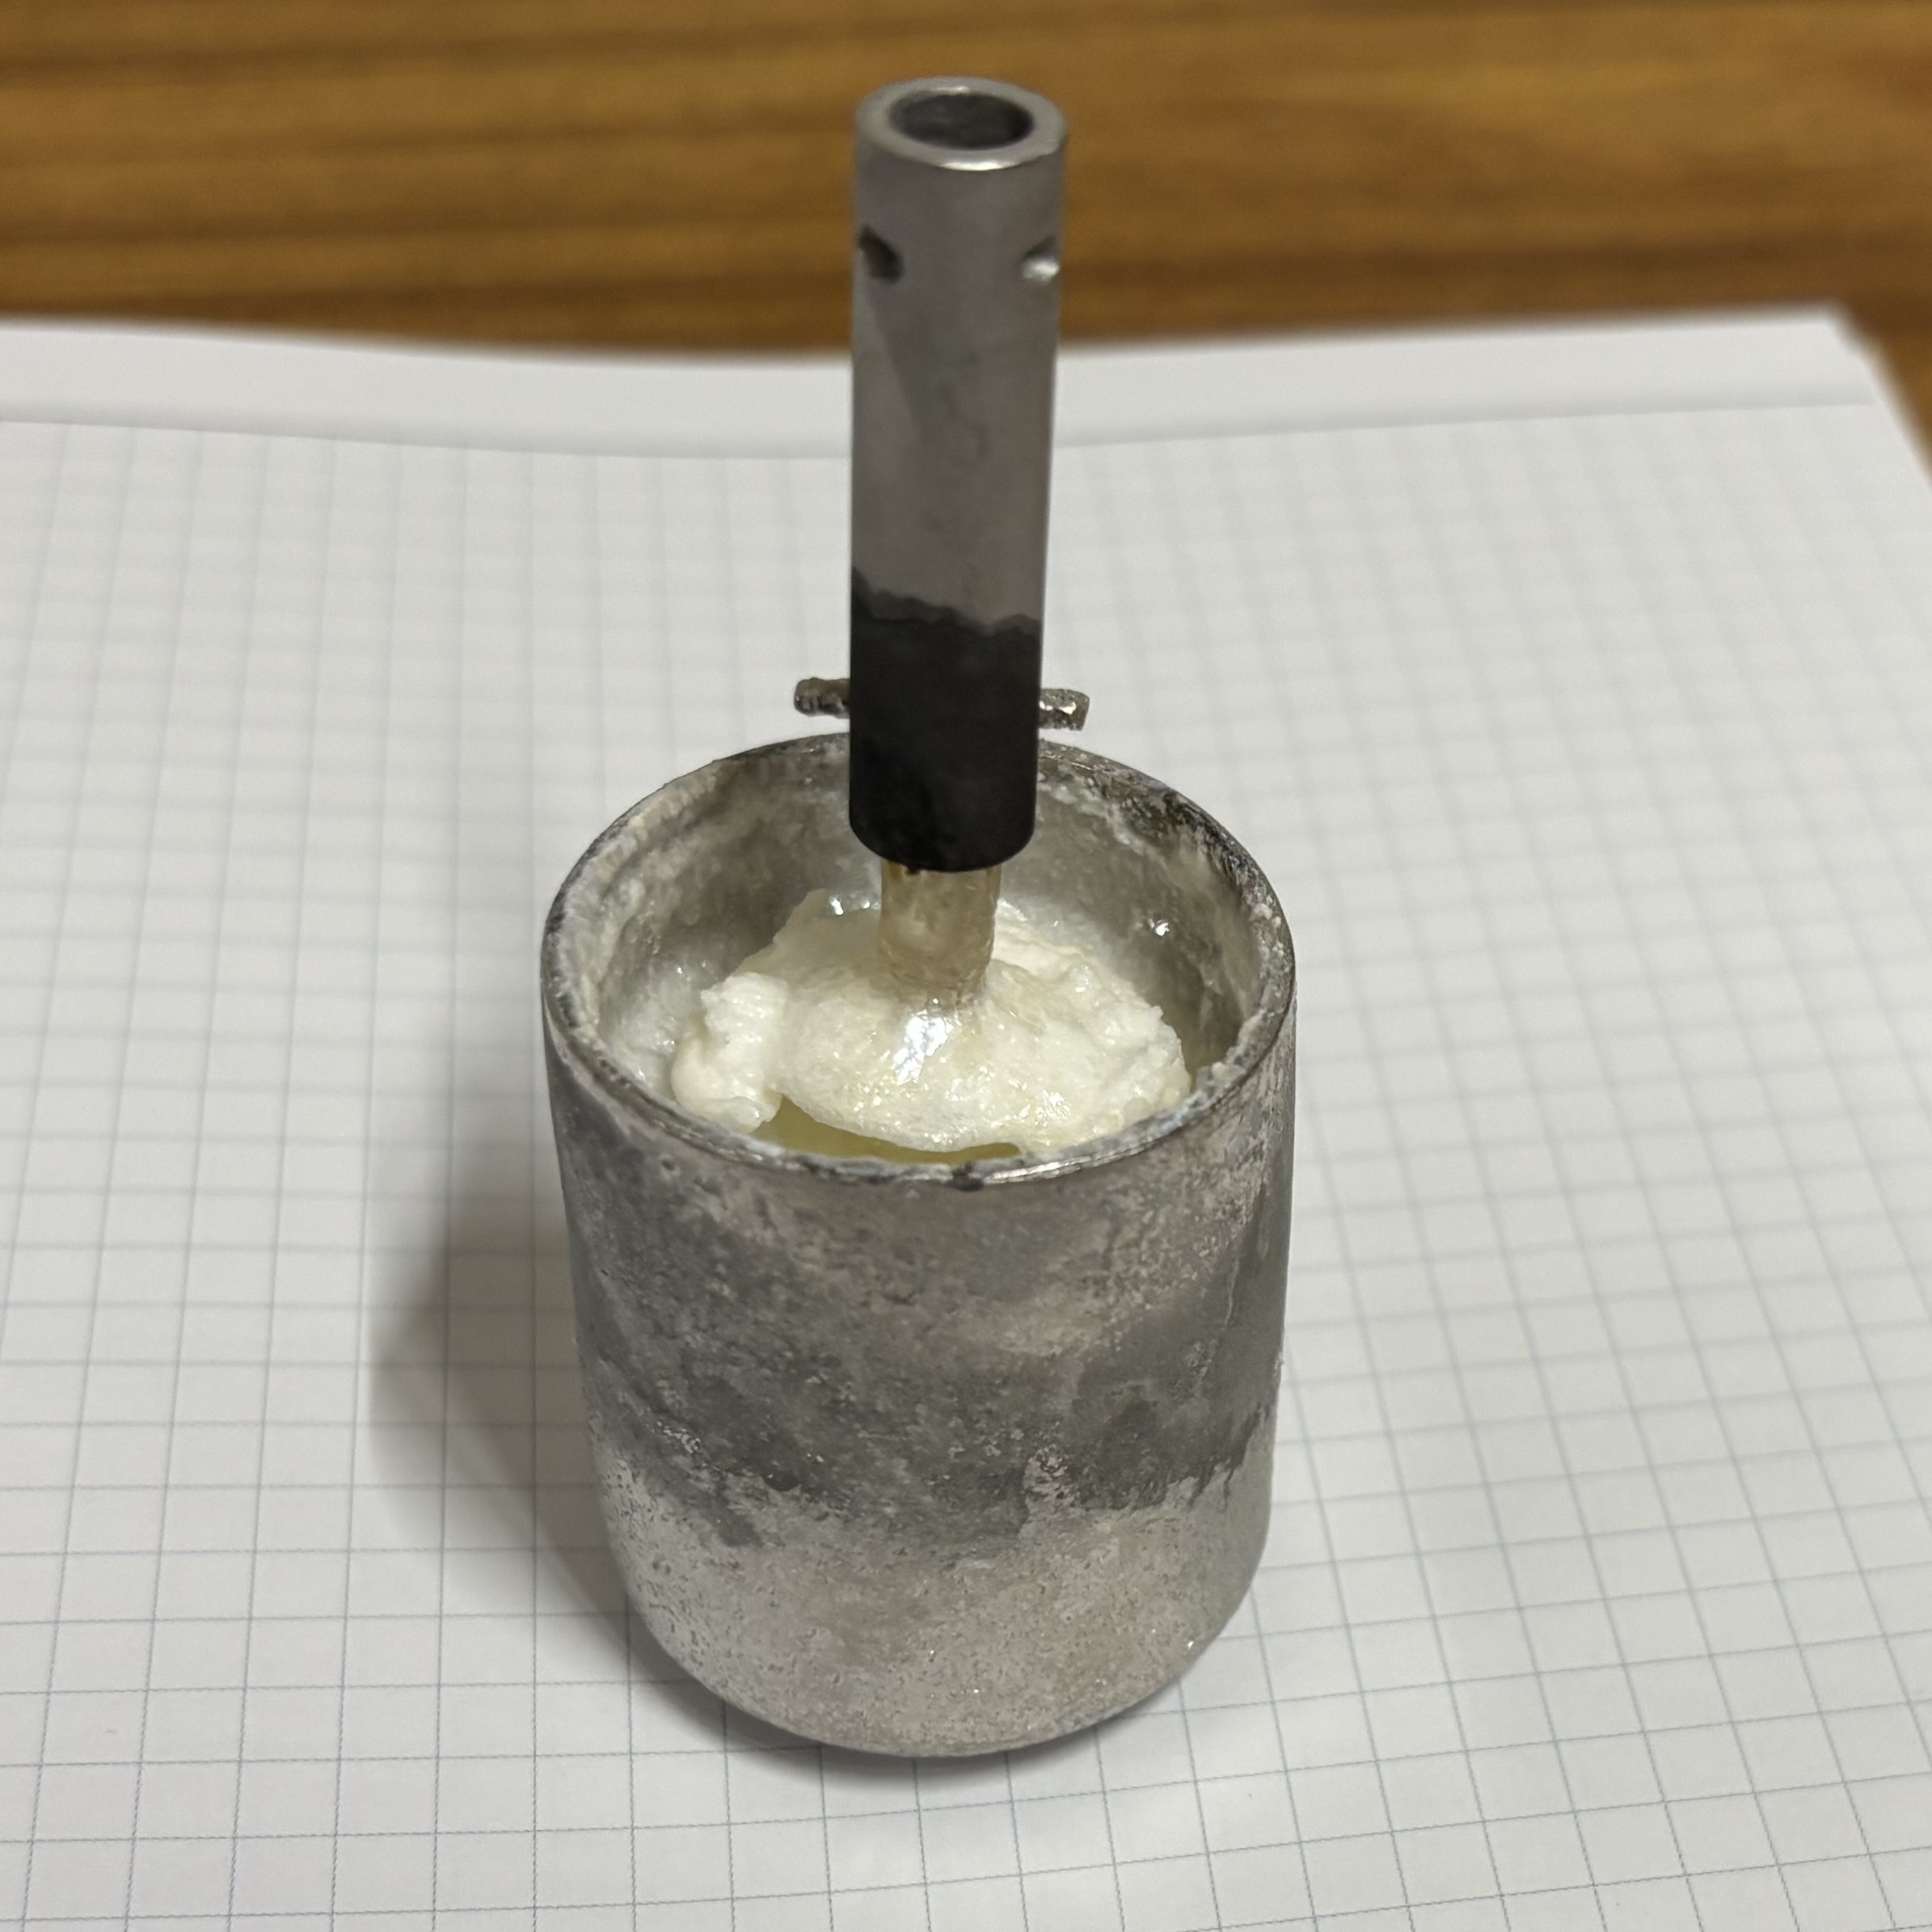
\includegraphics[width=\textwidth]{figures/Creuset avec agitateur.jpeg}
    \caption{Vue du creuset avec l'agitateur incrustée }
    \label{fig:img1}
\end{subfigure}
\hfill
\begin{subfigure}[b]{0.3\textwidth}
    \centering
    \includegraphics[width=\textwidth]{figures/Creuset YGG Vue de dessus.jpeg}
    \caption{Vue du creuset de dessus}
    \label{fig:img2}
\end{subfigure}
\hfill
\begin{subfigure}[b]{0.3\textwidth}
    \centering
    \includegraphics[width=\textwidth]{figures/vue agitateur.jpeg}
    \caption{Vue de l'agitateur une fois extrait}
    \label{fig:img3}
\end{subfigure}

\caption{Photographies du creuset et du germe attaché à l'agitateur}
\label{fig:photos_assemb}
\end{figure}
L’utilisation d’un microscope numérique KEYENCE a permis de mettre en évidence la présence de petits cristaux transparents sur les bords du creuset. La surface du mélange solidifié présente dans le creuset est inhomogène (transparente, vitreuse, blanc mat) (voir Figure \ref{fig:micro_assemb}).
\begin{figure}[H]
    \centering
    \includegraphics[width=0.4\linewidth]{figures/Creuset Flux Assemblage x20.jpg}
    \caption{Photographie au microscope numérique du creuset contenant le flux (grossissement x20)}
    \label{fig:micro_assemb}
\end{figure}

\subsubsection{Résultats DRX}
Après analyse des poudres extraites au bord du creuset et près du germe, la comparaison des deux diffractogrammes nous permet de conclure qu'il s'agit de la même phase cristalline qui a crû sur ces deux surfaces. (voir Annexe). En revanche il n'a pas été possible de détecter de trace du grenat YGG. 

\subsection{Résultats des essais de croissance dans différents flux}
À la sortie du four, des observations au microscope numérique ont été effectuées afin d’obtenir des images plus détaillées.

\begin{figure}[h]
\centering

\begin{subfigure}[b]{0.3\textwidth}
    \centering
    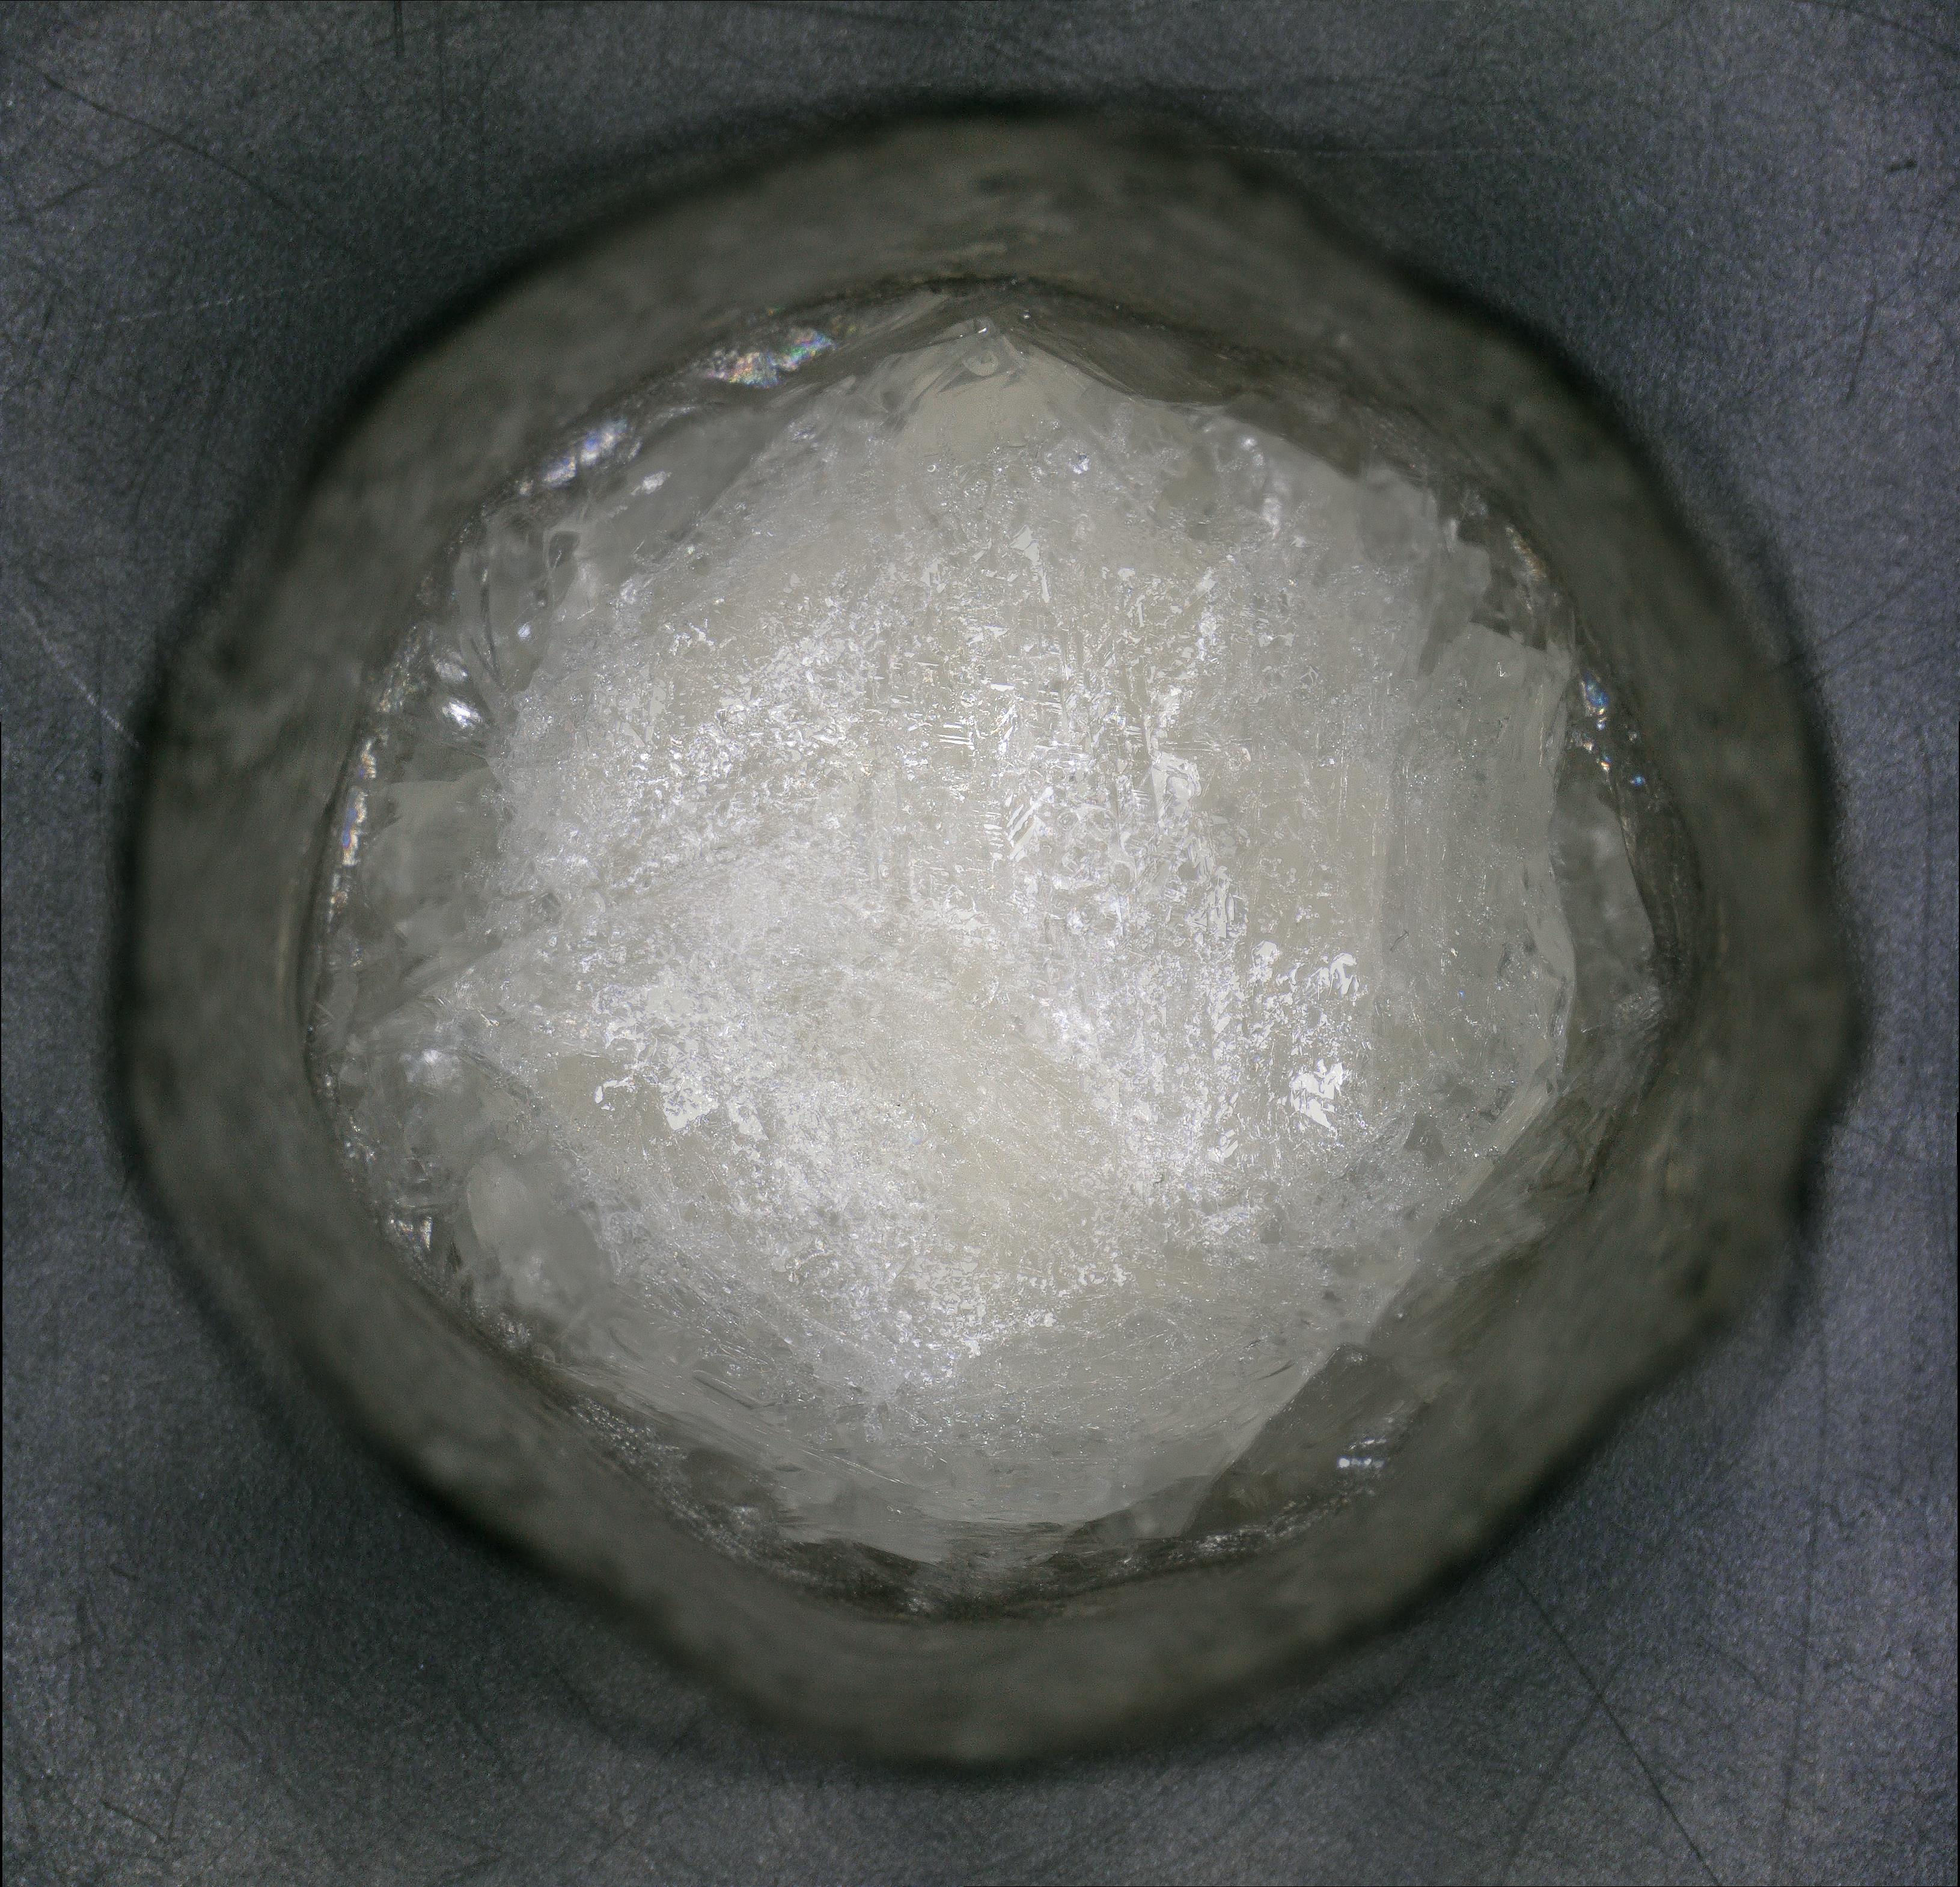
\includegraphics[width=\textwidth]{figures/Assemblage YGG x20.jpg}
    \caption{Vue du creuset [YGG] }
    \label{fig:img1}
\end{subfigure}
\hfill
\begin{subfigure}[b]{0.3\textwidth}
    \centering
    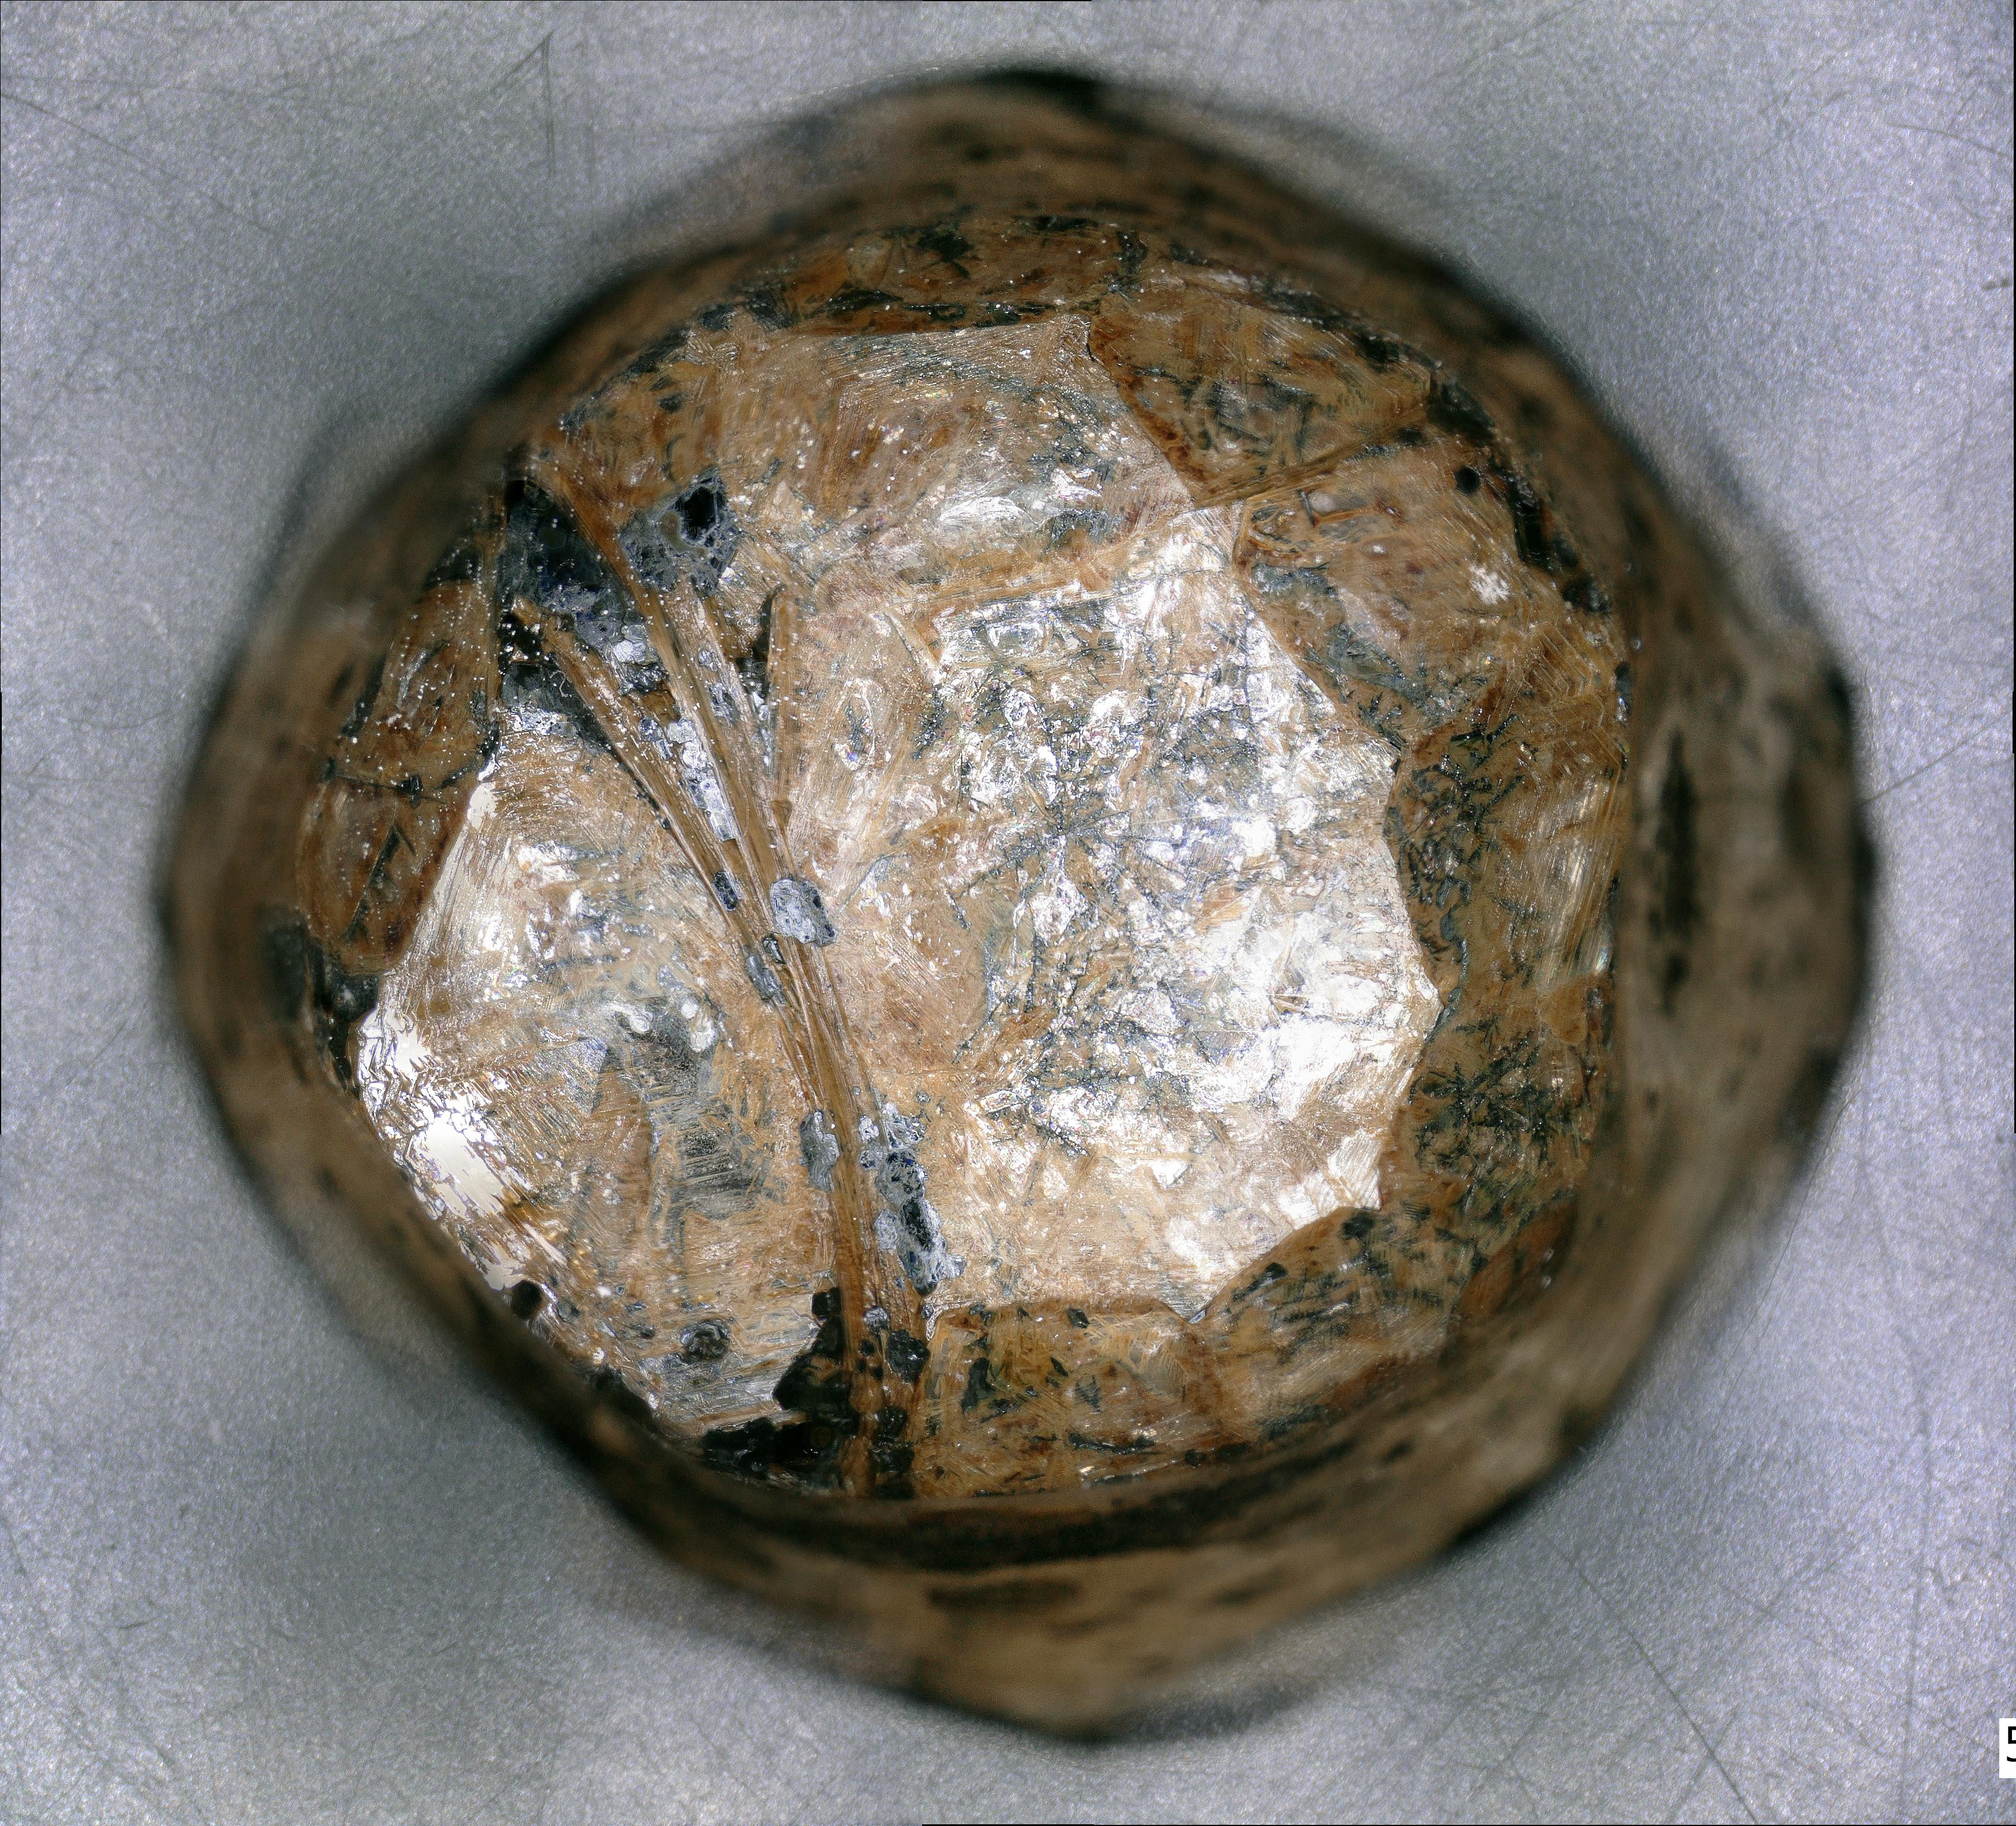
\includegraphics[width=\textwidth]{figures/Assemblage YIGG x20.jpg}
    \caption{Vue du creuset [YIGG]}
    \label{fig:img2}
\end{subfigure}
\hfill
\begin{subfigure}[b]{0.3\textwidth}
    \centering
    \includegraphics[width=\textwidth]{figures/Assemblage YIG x20.jpg}
    \caption{Vue du creuset [YIG]}
    \label{fig:img3}
\end{subfigure}

\caption{Photographie au microscope numérique des trois creusets après leur sortie du four (grossissement x20)}

\label{fig:photos_assemb}
\end{figure}

Le creuset [YIGG], apparaît translucide d'une teinte orangée avec la présence d'une certaine quantité de cristaux noirs hexagonaux à la surface. (Figure \ref{fig:YIGG-x50}

\begin{figure}
    \centering
    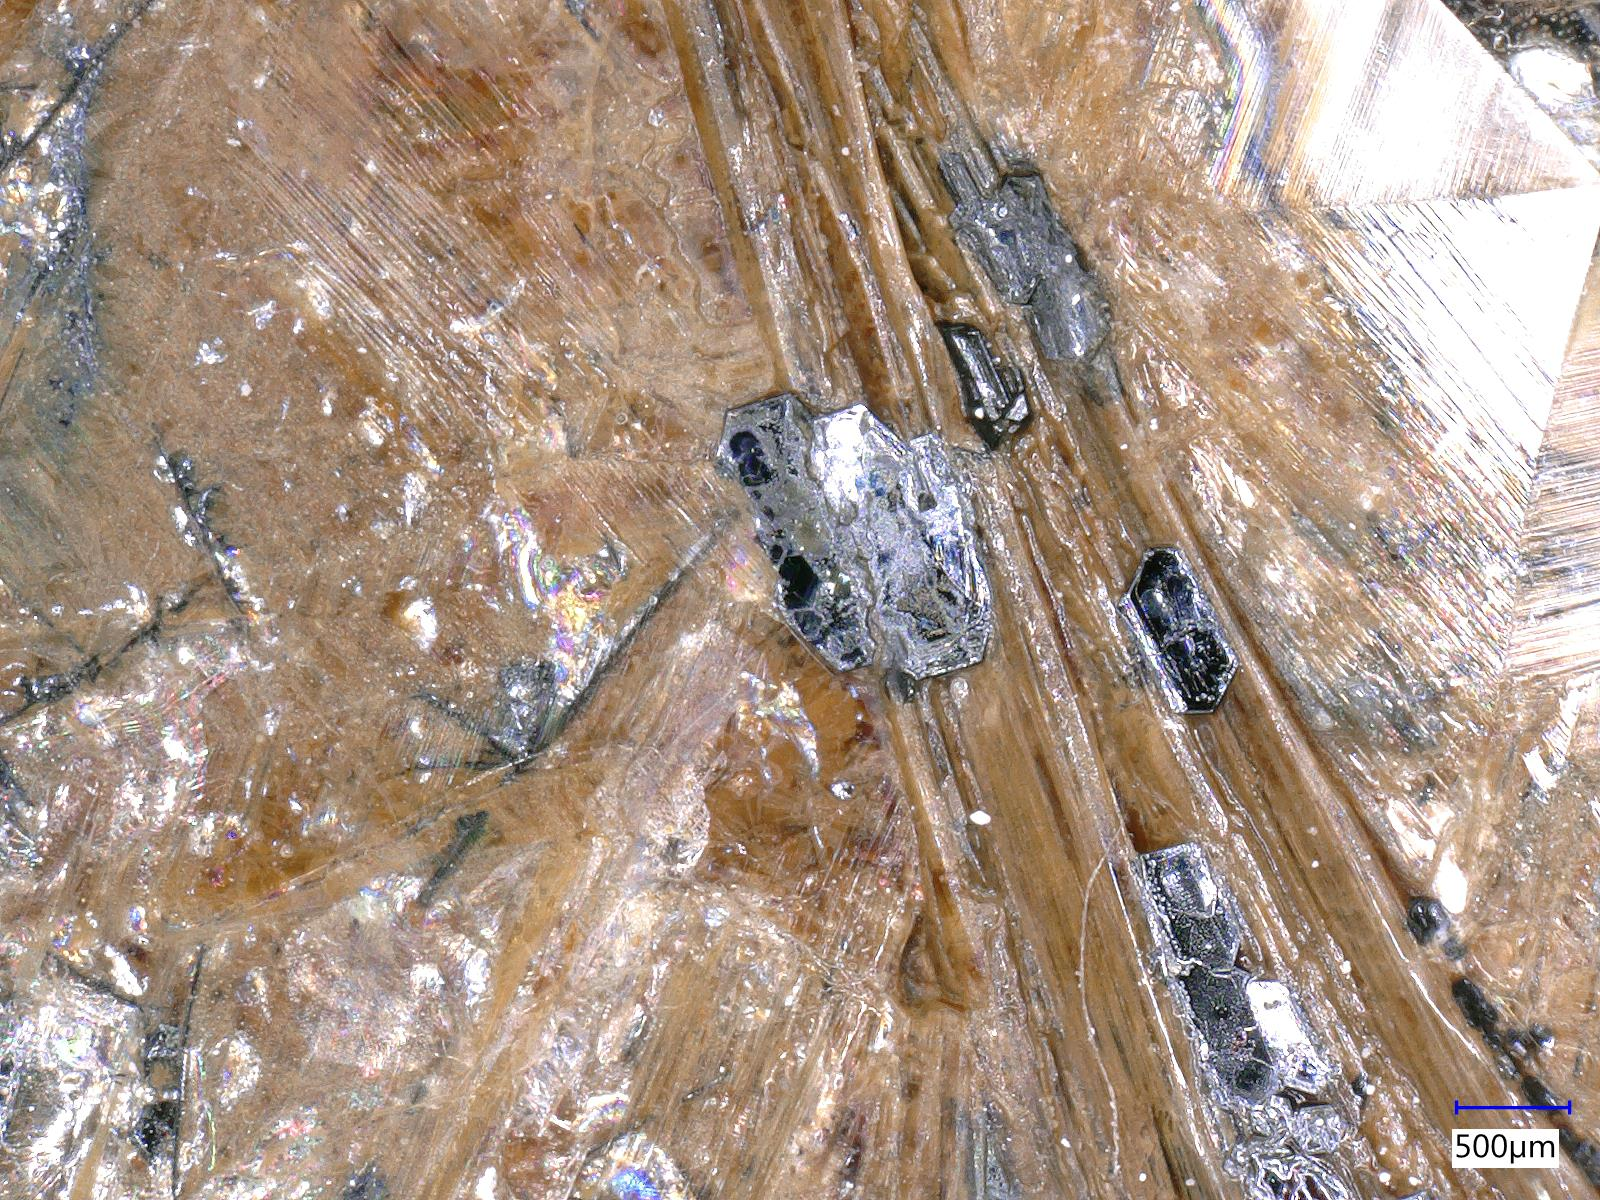
\includegraphics[width=0.5\linewidth]{figures/YIGG x50.jpg}
    \caption{Cristaux visibles à l’œil nu sur le creuset [YIGG] (grossissement x50)}
    \label{fig:YIGG-x50}
\end{figure}

Le contenu du creuset [YIG] est une phase opaque noire et striée (Figure \ref{fig:YIG_stries})à la surface. Elle laisse apparaître de faible tache rougeâtre lorsqu'elle est éclairée. On observe de petit cristaux noirs hexagonaux en surface (Figure \ref{fig:YIG_crist}). Bien que des cristaux noirs aient été observés, rien ne permet pour l’instant de confirmer qu’il s’agit de grenats. Cette hypothèse semble d’ailleurs peu probable compte tenu de la morphologie des cristaux présents dans les deux creusets. En effet, les grenats cristallisent selon un système cubique, tandis que les plaquettes hexagonales nettement visibles suggèrent une autre nature. En tenant compte des éléments présents dans le bain de cristallisation, ainsi que des résultats de DRX réalisés sur les échantillons extraits, ces cristaux pourraient appartenir à la famille des $BaFeO_{3-x}$.

\begin{figure}[h]
    \centering

    \begin{subfigure}[t]{0.45\textwidth}
        \centering
        \includegraphics[width=\textwidth]{figures/YIG x50.jpg}
        \caption{Vue des stries (grossissement x50)}
        \label{fig:YIG_stries}
    \end{subfigure}
    \hfill
    \begin{subfigure}[t]{0.45\textwidth}
        \centering
        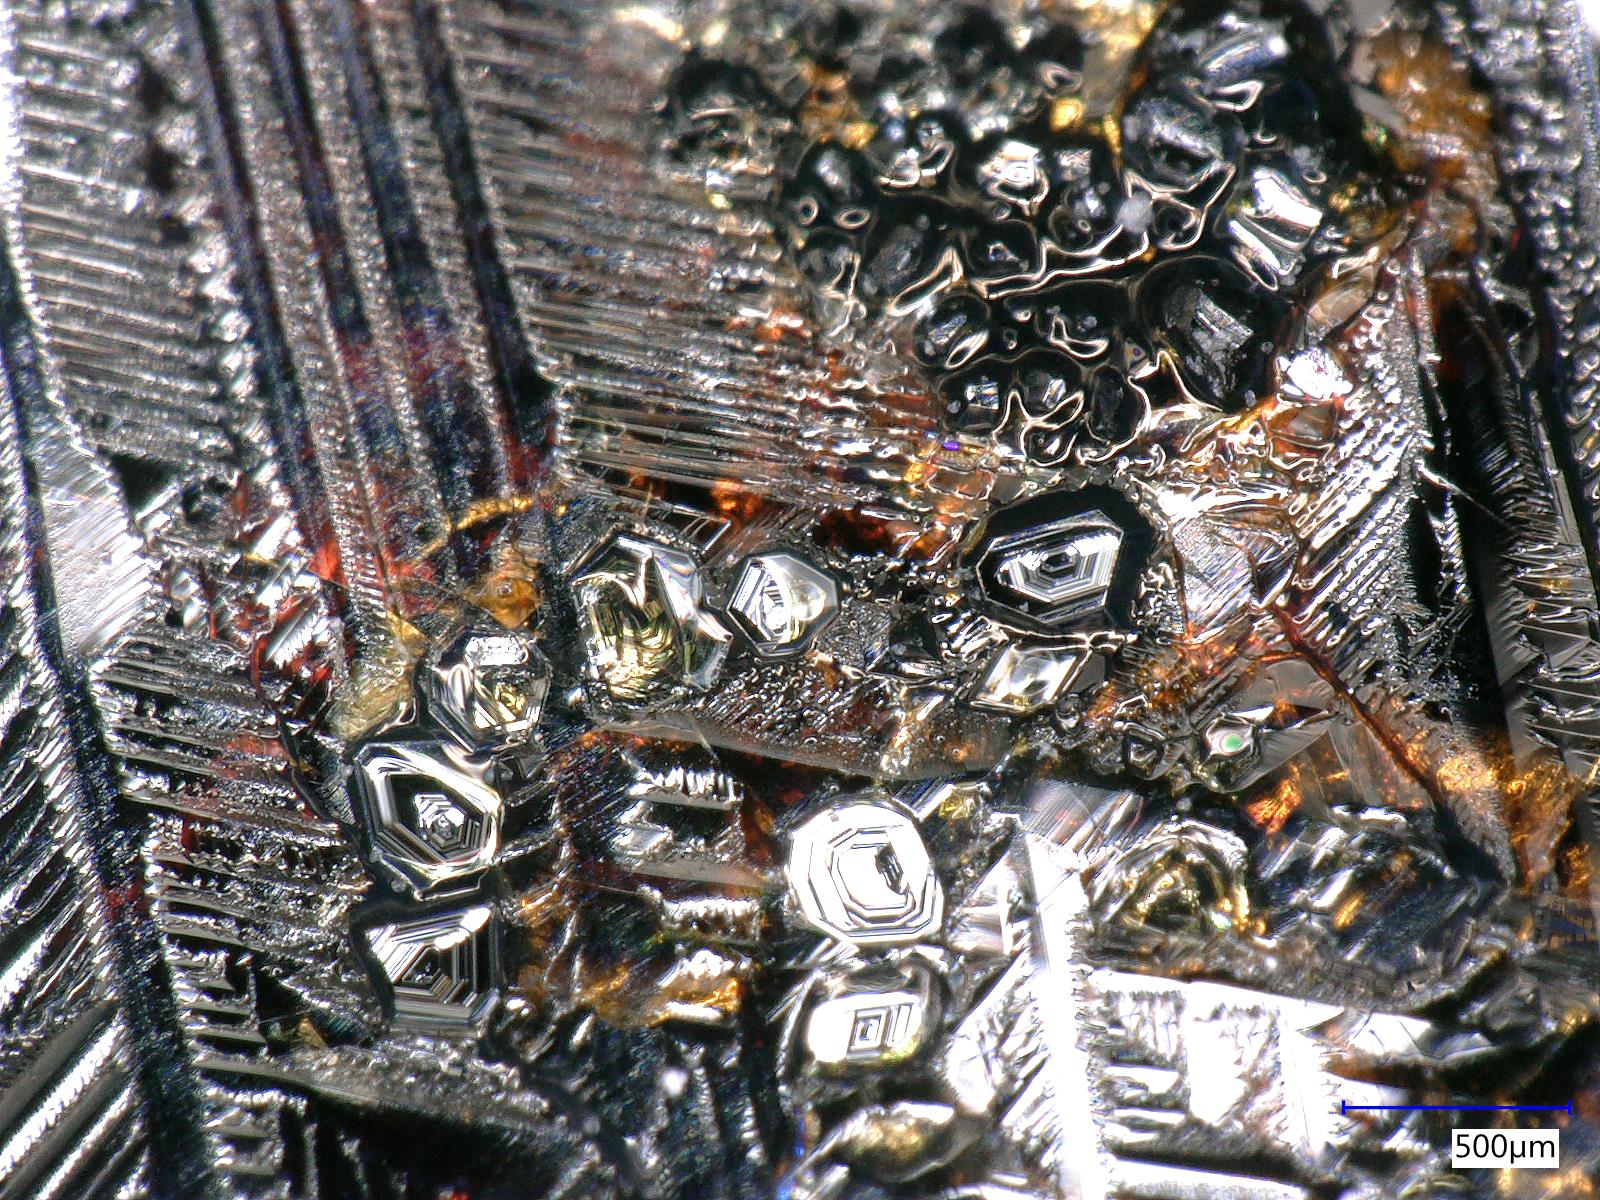
\includegraphics[width=\textwidth]{figures/YIG x100.jpg}
        \caption{Vue des cristaux hexagonaux (grossissement x100)}
        \label{fig:YIG_crist}
    \end{subfigure}

    \caption{Détails visible à la surface du creuset de [YIG]}
    \label{fig:detail_YIG}
\end{figure}

Le creuset [YGG] est composé d'une phase amorphe inhomogène translucide, transparente et blanche mat. On observe à la surface et dans les couches plus profondes des cristaux blanc ou transparent. Ainsi que des solides noirs opaques. (Figure \ref{fig:YGG-crist})

\begin{figure}[H]
    \centering
    \includegraphics[width=0.5\linewidth]{figures/YGG x100.jpg}
    \caption{Cristaux présent à la surface du creuset [YGG] et présence d'impuretées noires}
    \label{fig:YGG-crist}
\end{figure}

Les cristaux présents dans les trois creusets ont pu être récupéré dans le filtrat qui a suivi l'attaque acide des trois flux. Aussi, le creuset [YIG] possède après l'attaque acide un fond poly-cristallin composé de cristaux potentiellement cubique, donc éventuellement le grenat recherché.

\begin{figure}[H]
    \centering
    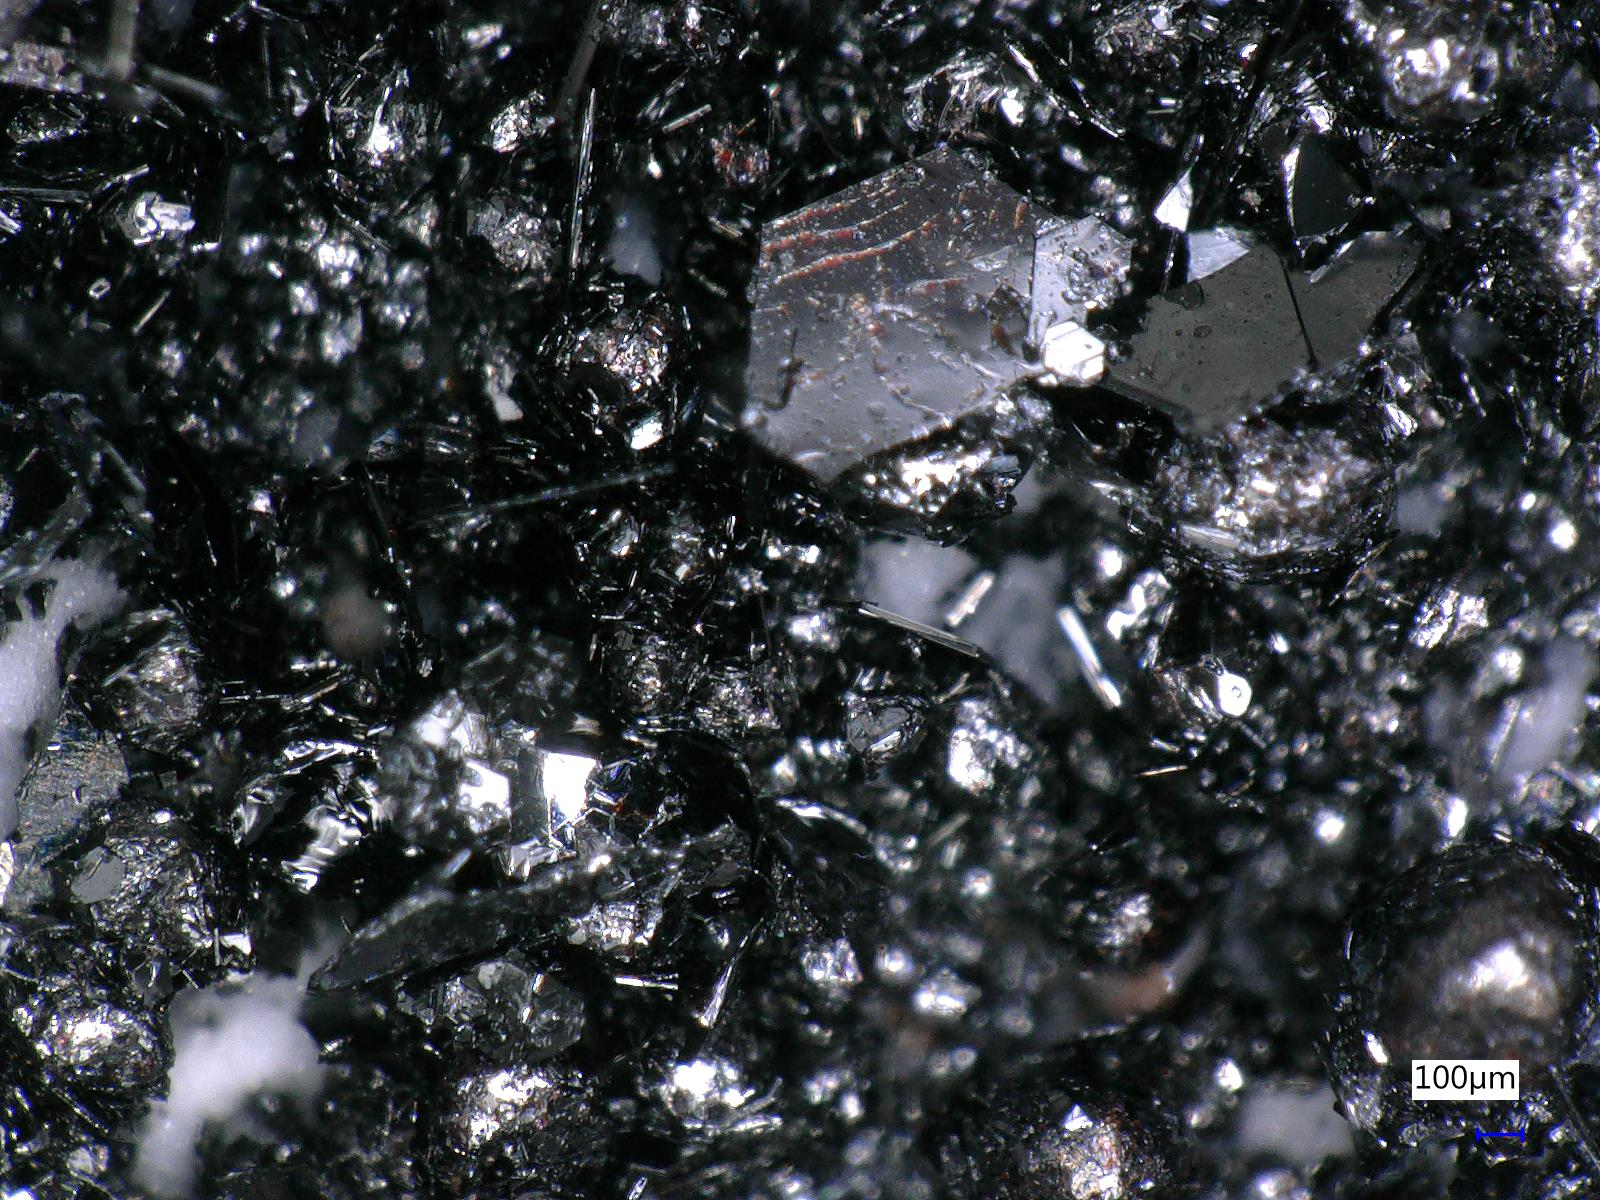
\includegraphics[width=0.5\linewidth]{figures/Creuset Post Acide YIGG x100.jpg}
    \caption{Cristaux au fond du creuset [YIG] après attaque acide}
    \label{fig:enter-label}
\end{figure}

Le filtrat du creuset [YGG] révèle des cristaux transparent ainsi qu'une phase amorphe blanc mat. On y aperçoit également des solides noirs mats. Tandis que le filtrat du creuset [YIGG] révèle une grande quantité de petit cristeux (moins d'1mm) noirs réfléchissant, ainsi que des cristaux blancs transparent, encore plus petit mais que l'on devine.
Enfin le filtrat du creuset [YIG] expose des amas de cristaux noirs plus volumineux, potentiellement cubique. Ceux-ci sont entourés d'une poudre verte, reste du flux et notamment du Fer ayant réagi avec l'acide nitrique (produit ferrique sous la forme $Fe^{2+}$). Tous ses détails sont visibles sur les différentes photographies de la Figure \ref{fig:micro_filtrats}.

\begin{figure}[H]
    \centering

    \begin{subfigure}[t]{0.3\textwidth}
        \centering
        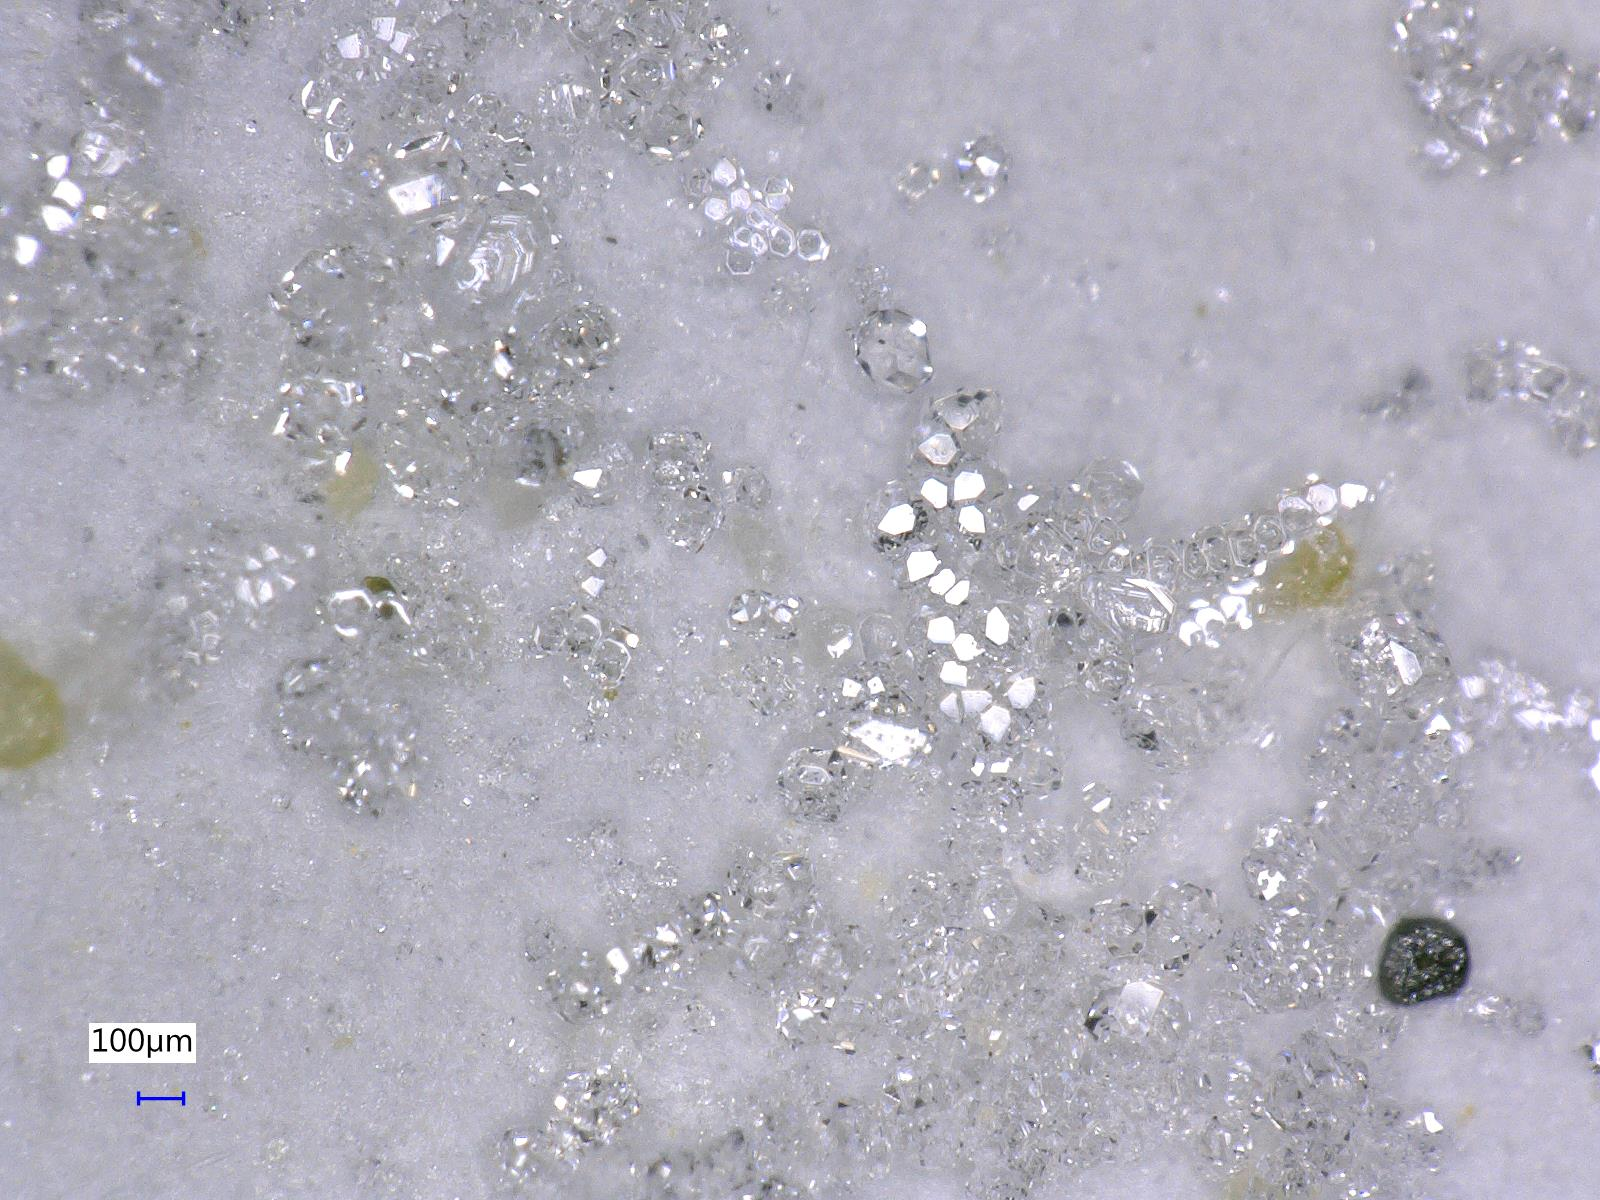
\includegraphics[width=\textwidth]{figures/Acide YGG x100.jpg}
        \caption{Vue du filtrat [YGG] (grossissement x100)}
        \label{fig:YGG_filtrat}
    \end{subfigure}
    \hfill
    \begin{subfigure}[t]{0.3\textwidth}
        \centering
        \includegraphics[width=\textwidth]{figures/Acide YIGG x50.jpg}
        \caption{Vue du filtrat [YIGG] (grossissement x100)}
        \label{fig:YIGG_filtrat}
    \end{subfigure}
    \hfill
    \begin{subfigure}[t]{0.3\textwidth}
        \centering
        \includegraphics[width=\textwidth]{figures/Acide YIG x200.jpg}
        \caption{Vue du filtrat [YGG] (grossissement x100)}
        \label{fig:YIG_filtrat}
    \end{subfigure}

    \caption{Photographie au microscope numérique des trois filtrats après attaque acide}
    \label{fig:micro_filtrats}
\end{figure}

\subsubsection{Résultats DRX}
Pour ce qui est des trois creuset à 7.5\% molaire de grenat, le diffractogramme du [YIG] est limpide : sa présence expliquant l'entièreté des pics. Le diffractogramme du creuset de [YIGG] confirme également la présence de YIG suspectée mais ne permet pas de confirmer la présence de YGG. Aussi on observe la présence de phases parasites celles-ci peuvent s'expliquer par la présence de nitrates présent dans le filtrat provenant de l’acide utilisé (acide nitrique $HNO_3$), qui a cristallisé avec les composés présents dans le flux. Le diffractogramme du creuset de [YGG] révèle des phases parasites similaires, et ne permet pas de confirmer la présence de YGG. 

Cependant la possibilité de croissance du grenat YGG dans ce flux est confirmé pour des proportions de YGG à 10\% molaire. Le diffractogramme du quatrième creuset révèle en effet la présence de ce grenat en plus d'une phase parasite $Ba(NO_3)_2$.

\section{Conclusion}
Ce stage s’est inscrit dans la continuité des recherches menées sur la croissance en flux des grenats d’yttrium, et plus particulièrement sur le YIG et le YGG. Il a permis de mettre en œuvre deux approches expérimentales : une tentative de croissance dirigée par tirage d’un monocristal de YGG, ainsi qu’une série d’essais dans différents flux afin d’étudier l’influence de la composition et de la concentration en grenat sur la cristallisation. Ces expériences ont mobilisé plusieurs techniques de préparation, de traitement chimique et de caractérisation (microscopie optique, attaque acide, diffraction par rayons X), qui ont permis d’observer et d’identifier les phases obtenues.

\subsection*{Résultats principaux}

La croissance dirigée d’un monocristal de YGG à partir d’un germe de $Gd_3Ga_5O_{12}$ n’a pas conduit à la formation de YGG, mais à celle d’une phase cristalline non identifiée. Cette tentative met en évidence les limites actuelles du protocole de tirage utilisé, probablement inadapté aux conditions de cristallisation du YGG. En parallèle, les essais réalisés dans des flux à base $BaO-B_2O_3-Na_2O$ ont permis de mieux cerner les conditions de croissance du YIG, qui se révèle relativement robuste et facilement identifiable par DRX.

Concernant le YGG, sa cristallisation a pu être confirmée dans le flux à base de sodium pour une concentration molaire de grenat portée à 10\%.  À des concentrations inférieures, aucune trace du YGG n’a pu être détectée. Quant au système mixte [YIGG], bien qu’il présente une grande variété de phases cristallisées, les diffractogrammes ne permettent pas de conclure à la présence conjointe des deux grenats, en raison d’un recouvrement de signaux et d’une possible compétition entre phases.

Les résultats obtenus montrent que la croissance en flux du grenat YGG est possible, mais nécessite une optimisation fine de la composition et des conditions expérimentales. L’augmentation de la concentration en grenat semble jouer un rôle clé dans la précipitation sélective de la phase souhaitée. Par ailleurs, la nature des phases parasites observées (notamment les composés nitrés issus de l’attaque acide) souligne l’importance de contrôler l’ensemble du protocole, y compris les traitements post-croissance.

Pour la suite, plusieurs pistes peuvent être envisagées : affiner la proportion des composants du flux, mieux contrôler le refroidissement, et explorer d’autres germes compatibles avec le YGG pour favoriser une croissance dirigée. 

\section{Bibliographie}
\begin{thebibliography}{17}

\bibitem{samuel}Rapport de stage de Samuel Collange à l'IRCP-MPOE, 2024 

\bibitem{mindat} Garnet Supergroup, Mindat, disponible sur : \url{https://www.mindat.org/min-1651.html}.

\bibitem{azo} Nd:YAG Lasers Properties and Applications, AZO optics, 2013, disponible sur : \url{https://www.azooptics.com/Article.aspx?ArticleID=470}.

\bibitem{chaneliere2014} Thierry Chanelière, A. Louchet-Chauvet, Alban Ferrier, Philippe Goldner, Cristaux et dispositifs optiques pour le traitement de l’information quantique, \textit{Techniques de l’ingénieur}, 2014.

\bibitem{musa2017} Makiyyu Abdullahi Musa, Raba’ah Syahidah Azis, Nurul Huda Osman, Jumiah Hassan, Tasiu Zangina, Structural and magnetic properties of yttrium iron garnet (YIG) and yttrium aluminum iron garnet (YAlG) nanoferrite via sol-gel synthesis, \textit{Elsevier}, 2017, disponible sur : \url{http://dx.doi.org/10.1016/j.rinp.2017.02.038}.

\bibitem{usami2011} N. Usami, Types of silicon–germanium (SiGe) bulk crystal growth methods and their applications, \textit{Elsevier}, 2011, disponible sur : \url{https://doi.org/10.1533/9780857091420.2.72}.

\bibitem{lohfeld2005} Stefan Lohfeld, M. Schütze, Oxidation behaviour of particle reinforced MoSi$_2$ composites at temperatures up to 1700°C. Part II: Initial screening of the oxidation behaviour of MoSi$_2$ composites, \textit{Materials and Corrosion}, 2005, disponible sur : \url{http://dx.doi.org/10.1002/maco.200403832}.

\bibitem{morris1979} A.W. Morris, D. Elwell, High temperature solution growth of yttrium aluminium garnet crystals using accelerated crucible rotation, \textit{Journal of Material Science}, 1979, disponible sur : \url{https://doi.org/10.1007/BF00688418}.

\bibitem{hiskes1974} R. Hiskes, LPE growth and characterization of magnetic garnets grown in BaO-based solvents, \textit{Journal of Crystal Growth}, 1974, disponible sur : \url{https://doi.org/10.1016/S0022-0248(74)80076-X}.

\bibitem{levin1949} Ernest M. Levin, Howard F. McMurdie, The system BaO-B$_2$O$_3$, \textit{Journal of the American Ceramic Society}, 1949, disponible sur : \url{http://dx.doi.org/10.1111/j.1151-2916.1949.tb18932.x}.

\bibitem{laudise1962} R.A. Laudise, R.C. Linares, E.F. Dearborn, Growth of Yttrium Iron Garnet on a Seed from a Molten Salt Solution, \textit{Journal of Applied Physics}, 1962, disponible sur : \url{https://doi.org/10.1007/978-1-4899-6391-8_144}.

\bibitem{elwell1974} D. Elwell, P. Capper, C.M. Lawrence, Viscosity and density of BaO/B$_2$O$_3$/BaF$_2$ fluxes and solutions, \textit{Journal of Crystal Growth}, 1974.

\bibitem{feigelson1990} R.S. Feigelson, R.J. Raymakers, R.K. Route, Growth of nonlinear crystals for frequency conversion, \textit{Progress in Crystal Growth and Characterization of Materials}, 1990, disponible sur : \url{https://doi.org/10.1016/0960-8974(90)90022-K}.

\bibitem{fedorov2002} P.P. Fedorov, A.E. Kokh, N.G. Kononova, Barium borate $\beta$-BaB$_2$O$_4$ as a material for nonlinear optics, \textit{Russian Chemical Reviews}, 2002, disponible sur : \url{http://dx.doi.org/10.1070/RC2002v071n08ABEH000716}.

\bibitem{timofeeva1981} V.A. Timofeeva, A.B. Bykov, V.S. Nikolov, Phase equilibria in BaO-B$_2$O$_3$-BaF$_2$-Y$_2$O$_3$-Fe$_2$O$_3$ system, \textit{Journal of Crystal Growth}, 1981, disponible sur : \url{https://doi.org/10.1016/0022-0248(81)90354-7}.

\bibitem{suemune1974} Y. Suemune, N. Inoue, Crystallization of garnets in BaO-BaF$_2$-B$_2$O$_3$ solvents, \textit{Journal of Crystal Growth}, 1974, disponible sur : \url{https://doi.org/10.1016/0022-0248(74)90397-2}.

\bibitem{capper1974} P. Capper, D. Elwell, Appraisal of BaO/B$_2$O$_3$/BaF$_2$ fluxes for the growth of yttrium aluminium garnet, \textit{Journal of Crystal Growth}, 1974, disponible sur : \url{https://doi.org/10.1016/0022-0248(74)90202-4}.

\end{thebibliography}
\newpage
\section{Annexes}
\setcounter{figure}{0}
\appendix
\section{Programmation des fours}
\label{annexe:programme_four}
\begin{figure}[p]
    \centering
    \includegraphics[width=\textwidth,keepaspectratio]{figures/Programme_temp_flux.png}
    \caption{Programme du four pour le flux $0.4BaO - 0.3B_2O_3 - 0.3BaF_2$}
    \label{fig:programme_temp_flux}
\end{figure}
\begin{figure}[p]
    \centering
    \includegraphics[width=\textwidth,keepaspectratio]{figures/Programme_temp_flux.png}
    \caption{Programme du four pour le flux $0.4BaO - 0.3B_2O_3 - 0.3BaF_2$}
    \label{fig:programme_temp_flux}
\end{figure}
\newpage
\section{Résultats DRX}
\begin{figure}[htbp]
    \centering
    \includegraphics[width=\textwidth]{figures/Ka1_spin_flux433_4pcYGG_centre et bord.pdf}
    \caption{Comparaison entre les diffractogrammes des échantillons récoltés sur le germe (bleu) et au bord du creuset (rouge)}
    \label{fig:exemple-pdf}
\end{figure}

\begin{figure}[htbp]
    \centering
    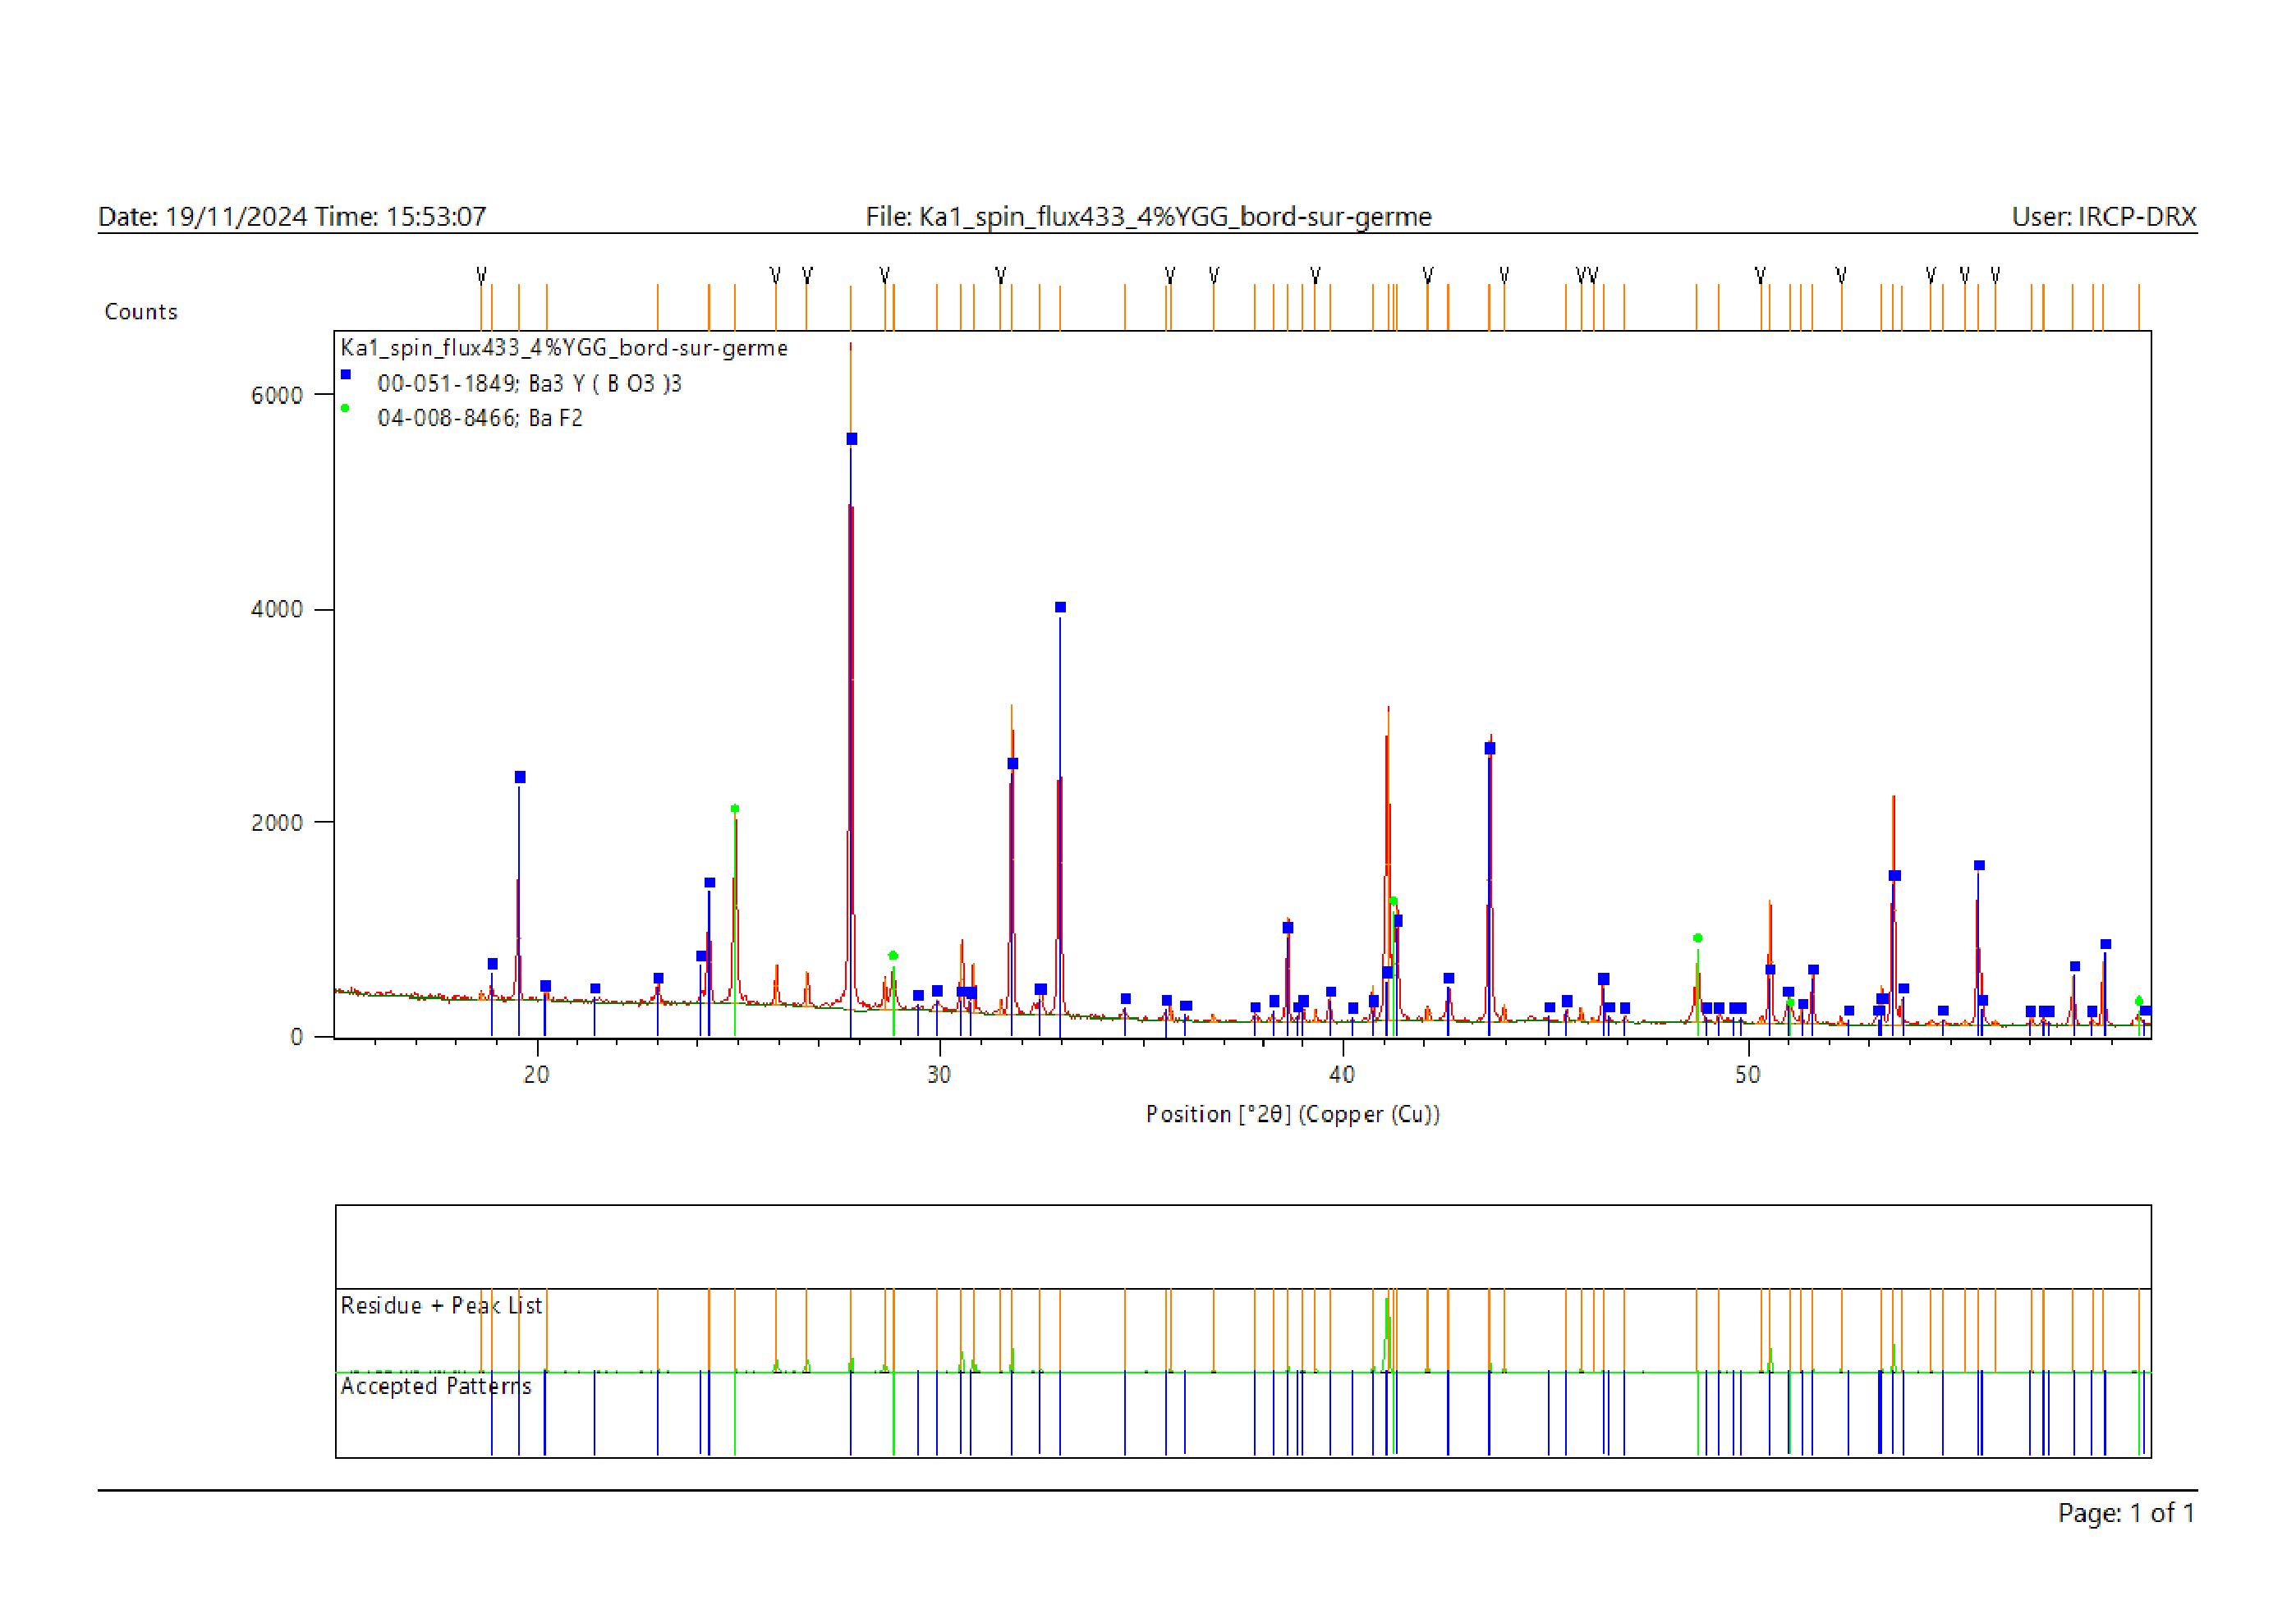
\includegraphics[width=\textwidth]{figures/Ka1_spin_flux433_4pcYGG_bord-sur-germe.pdf}
    \caption{Diffractogramme des cristaux présent au bord du creuset de tirage}
    \label{fig:exemple-pdf}
\end{figure}

\begin{figure}[htbp]
    \centering
    \includegraphics[width=\textwidth]{figures/Ka1_spin_flux433_4pcYGG_centre-sur-germe.pdf}
    \caption{Diffractogramme des cristaux présent sur le germe du creuset de tirage}
    \label{fig:exemple-pdf}
\end{figure}

\begin{figure}[htbp]
    \centering
    \includegraphics[width=\textwidth]{figures/Ka1_spin_flux433_4pccreusetYIGG.pdf}
    \caption{Diffractogramme des cristaux formés dans le creuset [YIGG]}
    \label{fig:exemple-pdf}
\end{figure}

\begin{figure}[htbp]
    \centering
    \includegraphics[width=\textwidth]{figures/Ka1_spin_flux433_4pccreusetYIG.pdf}
    \caption{Diffractogramme des cristaux formés dans le creuset [YIG]}
    \label{fig:exemple-pdf}
\end{figure}

\end{document}
  